% No need to change the first 4 lines of this file
\documentclass{uicthesi}

% This is the user manual for UICTHESI CLS, originally found
% at https://www.math.uic.edu/graduate/current/uicthesi, and
% modified by Pete Snyder <snyder@gmail.com> to match the
% current department requirements.
\usepackage{booktabs}
\usepackage{listings}
\usepackage{newlfont}
\usepackage{amsfonts}
\usepackage{amssymb}
\usepackage[xindy={glsnumbers=false},nonumberlist,acronym,nopostdot,nogroupskip,nomain]{glossaries}
\usepackage{xspace}
\usepackage[htt]{hyphenat}
\usepackage{float}
\usepackage{flushend}
\usepackage{footnote}
\usepackage{enumitem}
\usepackage{url}
\usepackage{caption}
\usepackage{graphicx}
\usepackage{amsmath,,amsthm,stmaryrd,paralist,tikz,amsthm}
\usepackage[mathscr]{euscript}
\usetikzlibrary{matrix,arrows,decorations.pathmorphing}

\usepackage{hyperref}
\hypersetup{
pdfauthor={Keaton Quinn},
pdftitle={Asymptotically Poincar\'e surfaces in quasi-Fuchsian manifolds},
colorlinks=true,linkcolor=verydarkblue,
citecolor=verydarkblue,urlcolor=verydarkblue
}

\newglossarystyle{clong}{%
 \renewenvironment{theglossary}%
     {\begin{longtable}{p{.2\linewidth}p{.8\linewidth}}}%
     {\end{longtable}}%
  \renewcommand*{\glossaryheader}{}%
  \renewcommand*{\glsgroupheading}[1]{}%
  \renewcommand*{\glossaryentryfield}[5]{%
    \glstarget{##1}{##2} & ##3\glspostdescription\space ##5\\}%
  \renewcommand*{\glossarysubentryfield}[6]{%
     & \glstarget{##2}{\strut}##4\glspostdescription\space ##6\\}%
  %\renewcommand*{\glsgroupskip}{ & \\}%
}

\makesavenoteenv{tabular}
\makesavenoteenv{table}

% See https://www.ctan.org/pkg/glossaries for questions on this package.
% Refer to the acronyms you define here as \gls{nyc}.
%
% This make sure that this text:
%    The Ramones are from \gls{nyc}, thats right, \gls{nyc}.
% Gets output like this:
%    The Ramones are from New York City (NYC), thats right, NYC.
% And that a line in the acronyms section of your thesis has an entry like:
%    NYC         New York City
\newacronym{nyc}{NYC}{New York City}
\newacronym{rtr}{RTR}{Rocket to Russia}
\newacronym{eofc}{EOFC}{End of the Century}
\def\new@fontshape#1#2#3#4#5{\expandafter
     \edef\csname#1/#2/#3\endcsname{\expandafter\noexpand
                                 \csname #4\endcsname}}
\new@fontshape{cmr}{bx}{sc}{
      <5>cmcsc8 at 5pt%
      <6>cmcsc8 at 6pt%
      <7>cmcsc8 at 7pt%
      <8>cmcsc8%
      <9>cmcsc9%
      <10>cmcsc10%
      <11>cmcsc10 at 10.95pt%
      <12>cmcsc10 at 12pt%
      <14>cmcsc10 at 14.4pt%
      <17>cmcsc10 at 17.28%
      <20>cmcsc10 at 20.736pt%
      <25>cmcsc10 at 24.8832pt%
      }{}
\mathversion{normal}
\newcommand{\ams}{{$\cal{A}\cal{M}\cal{S}$}}
\newcommand{\amslatex}{{$\cal{A}\cal{M}\cal{S}$-\LaTeX{}}}
\newcommand{\amstex}{{$\cal{A}\cal{M}\cal{S}$-\TeX{}}}
\newcommand{\BibTeX}{{\rm B\kern-.05em{\sc i\kern-.025em b}\kern-.08em
    T\kern-.1667em\lower.7ex\hbox{E}\kern-.125emX}}
\newcommand{\uicthesi}{{$\mathbb{UICTHESI}$}}

\newcommand\bs{\char '134 }   % A backslash character for \tt font
\newcommand{\lb}{\char '173 } % A left brace character for \tt font
\newcommand{\rb}{\char '175 } % A right brace character for \tt font

% one or two other commands
\def\newfont#1#2{\@ifdefinable #1{\font #1=#2\relax}}
\def\symbol#1{\char #1\relax}

\makeglossaries

% Use this file to include custom commands...
\newcommand{\R}{\mathbb{R}}
\newcommand{\Q}{\mathbb{Q}}
\newcommand{\Z}{\mathbb{Z}}
\newcommand{\C}{\mathbb{C}}
\newcommand{\N}{\mathbb{N}}
\newcommand{\D}{\mathbb{D}}
\newcommand{\T}{\mathbb{T}}
\newcommand{\RP}{\mathbb{R}\mathrm{P}}
\newcommand{\CP}{\mathbb{C}\mathrm{P}}
\renewcommand{\H}{\mathbb{H}}
\let\oldS\S
\renewcommand{\S}{\mathbb{S}}
\newcommand{\s}{\mathbb{S}}


\newtheorem{thm}{Theorem}[section]
\newtheorem*{thm*}{Theorem}
\newtheorem{lem}[thm]{Lemma}
\newtheorem*{lem*}{Lemma}
\newtheorem{cor}[thm]{Corollary}
\newtheorem*{cor*}{Corollary}
\newtheorem{prop}[thm]{Proposition}
\newtheorem*{prop*}{Proposition}
\newtheorem{defn}{Definition}
\newtheorem*{defn*}{Definition}
\newtheorem{question}{Question}
\newtheorem*{question*}{Question}

\newtheorem{bigthm}{Theorem}
\renewcommand{\thebigthm}{\Alph{bigthm}}

\newcommand{\del}{\nabla}
\newcommand{\two}{I\!\!I}



\begin{document}

% The title of the thesis
\title{Limits of Foliations in Quasi-Fuchsian Manifolds
%\begin{center} {\sf \color{red} DRAFT VERSION 4 --- {\today} } \end{center}
}


% Your full name
\author{Keaton Quinn}

% Mention all degrees you hold currently
\pdegrees{B.S., Michigan State University, 2014}

% Probably no need to edit this
\degree{Doctor of Philosophy in Mathematics}

% Add your committee members, one per line, mentioning external universities
% where relevant
\committee{David Dumas, Chair and Advisor \\
Daniel Groves \\
Julius Ross \\
Laura Schaposnik \\
Benson Farb, University of Chicago}

% No need to make any changes to the next 10 lines
\maketitle
\copyrightpage
%\dedication

A brief dedication to someone you care about.  For example, ``Dedicated to
my cats, Neo and Trinity, who are purrfect in every way.''.

An example of ``Dedication'' can be found on page 15 of the thesis
manual\footnote{\url{http://grad.uic.edu/sites/default/files/pdfs/ThesisManual_rev_06Oct2016.pdf}}.
\acknowledgment

I would like to start by thanking my advisor David Dumas.
I thank him for suggesting this project, for indulging my preferred mathematical viewpoints, for his many comments and suggestions on drafts of my mathematical papers, and for his guidance.

I gratefully acknowledge the support of the National Science Foundation. Specifically, my research was partially funded by DMS-1246844, RTG: Algebraic and Arithmetic Geometry, at the University of Illinois at Chicago and DMS-1709877, Character Varieties and Locally Homogeneous Geometric Structures. 
I also acknowledge support from U.S. National Science Foundation grants DMS 1107452, 1107263, 1107367 ``RNMS: Geometric Structures and Representation Varieties" (the GEAR Network).
The GEAR network funded my trip to the University of Luxembourg where I met with Jean-Marc Schlenker. 
I thank him for helpful conversations and research suggestions.
I also thank his graduate students, including Filippo Mazzoli, for their hospitality.  

I would also like to thank the mathematics graduate students for making the University of Illinois at Chicago an enjoyable place to learn. 
I am grateful for GGTDS, grateful to Sam Dodds for our many rambling mathematical musings, and thankful to Hunter Chase for commiserating with me. 
Special thanks go to Charles Alley, J\=anis Lazovskis, and Nathan Lopez for their friendship and support, for our weekly research seminar, and for their inspiration.
In particular, I thank Charles for keeping me grounded in reality, I thank Nathan for his companionship, and I thank J\=anis for putting up with me as a roommate for five years. 
Thanks also go to the administrative staff of the Department of Mathematics, Statistics, and Computer Science for keeping everything running. This includes but is not limited to Lisa Jones, Maureen Madden, and Eloy Reyes.

I thank Hanni Nichols for inspiring me to pursue mathematics, for prodding me towards graduate school, for reassuring me, for believing in me, and for her friendship.
I also thank my family, Keith Quinn, Sandra Quinn, Taylor Quinn and Rom\'an Rampinini, who have been nothing but supportive. 
And finally, I thank Irving Daniel Sandoval Gonzalez for being so inspiring, motivating, supportive, and understanding, and for helping me make it to the end.


% This line is required, but of course replace my initials with yours.
\initials{KPQ}
%\authorcontributions

This section should give a rough overview of each chapter in the thesis,
highlighting your contributions.  Most importantly, for each one of your
papers you are quoting, this section should briefly describe what each author's
role / contribution was.

An example of ``Contribution of Authors'' section is on page 3 of the
University's guide to iThenticate\footnote{\url{http://grad.uic.edu/sites/default/files/pdfs/Introduction_to_Screening_Your_Thesis_or_Dissertation_using_iThenticate-final_a.pdf}}.
\tableofcontents
%\listoftables
%\listoffigures
\printglossary[type=\acronymtype,title=LIST OF ABBREVIATIONS,style=clong]
\summary

We study the asymptotic behavior of certain foliations of ends of quasi-Fuchsian manifolds. 
We introduce a class of such foliations, which we call asymptotically Poincar\'e families as they are asymptotic to a family of surfaces determined naturally by the Poincar\'e metric on the Riemann surface at infinity.
We prove the limiting behavior of any asymptotically Poincar\'e family is completely determined by the geometry of the quasi-Fuchsian manifold $M$ and the conformal structure on the ideal boundary of $M$. 
Specifically, the conformal classes of the first and second fundamental forms $[I_\epsilon]$ and $[\two_\epsilon]$ of the surfaces in an asymptotically Poincar\'e family converge in Teichm\"uller space as $\epsilon \to 0$ to the conformal structure of the surface at infinity of the end of $M$.
At $\epsilon  = 0$, the tangent vectors satisfy $\dot{[I_\epsilon]} = c \mathrm{Re}(\phi)$ and $\dot{[\two_\epsilon]} = 0$ where $\phi$ is the holomorphic quadratic differential of the complex projective structure at infinity and $c$ a constant that depends on the foliation. 

As an application of these results we establish a conjecture of Labourie regarding the asymptotic behavior of the $k$-surface foliation he constructs in \cite{labourie1992}.
We also show that the constant mean curvature foliation of Mazzeo and Pacard \cite{mazzeo-pacard2011} forms an asymptotically Poincar\'e family and so we can describe its asymptotics as well.


% This is where you write the paper.  I've included a sample chapter
% below, to suggest a possible organization.  Just add references to the
% rest of your paper here.
\chapter{Epstein Surfaces}
\label{epstein-surfaces}

\section{The visual metric construction}


A natural trivialization of the unit tangent bundle of hyperbolic space $U\H^3$ is given as
\[
U\H^3 \to \H^3 \times \CP^1
\quad \text{ by } \quad
(p,v) \mapsto (p, \lim_{t \to \infty} \exp_p (tv) ).
\]
That is we map $(p,v)$ to the ideal endpoint of the geodesic ray through $p$ in the direction $v$. 
Restricting to a point $p$ and using the diffeomorphism $U_p\H^3 \to \CP^1$, we can push forward to $\CP^1$ the induced metric on $U_p\H^3$ considered as a submanifold of $T_p\H^3$ with metric given by the inner product $g_{\H^3}(p)$. 
The resulting metric $V_p$ on $\CP^1$ is called the visual metric from $p$.
As an example, the visual metric from the origin in the ball model $V_0$ is just the spherical metric $\overset{\circ}{\sigma}$ on $S^2$ (which is identified with $\CP^1$ in this model). 
In general, if $M \in \mathrm{PSL}_2\C$ is an isometry taking $0$ to the point $p$, then $V_p = M_*V_0$. 

As the spherical metric belongs to the conformal class of $\CP^1$, we have that $V_0$ is a conformal metric. 
Since M\"obius transformations are biholomorphisms of $\CP^1$, each $V_p$ is also a conformal metric. 
If we work in the ball model of hyperbolic space $\H^3 \cong \mathbb{B}^3$ we can actually be explicit regarding the conformal factor between $V_p$ and $\overset{\circ}{\sigma}$ using the affine parameter of a horosphere. 
If $H$ is a horosphere, then its affine parameter is the signed hyperbolic distance from $0 \in \H^3$ to $H$, positive if $0$ is outside $H$ and negative if inside. 
Then for $p \in \H^3$ there is a unique horosphere based at $z \in \CP^1$ that contains $p$. 
Denote by $[p,z]$ the affine parameter of this horosphere. 
Then
\[
V_p(z) = e^{2[p,z]}\overset{\circ}{\sigma}(z).
\]

We now describe the Visual Metric Construction (see \cite{anderson1998}). 
This is a process that, given a strictly convex surface $S$ in $\H^3$, gives a domain $\Omega$ in $\CP^1$ and a conformal metric $\sigma$ on $\Omega$.
The idea is this: Given $S$, we have its image under the Gauss map on $\CP^1$. 
That is, given a unit normal vector field $n$ on $S$ for which $S$ is strictly convex, define
\[
\mathcal{G}:S \to \CP^1 \text{ by } \mathcal{G}(p) = \lim_{t \to \infty} \exp_p(t n(p)).
\]
The strict convexity of $S$ guarantees the map $\mathcal{G}$ is a local homeomorphism. 
We assume now that it is actually a homeomorphism.
The image surface also comes equipped with a metric $\sigma$ by defining $\sigma(\mathcal{G}(p)) = V_p(\mathcal{G}(p))$. 
Since for each $p$ the visual metric from $p$ is a conformal metric on $\CP^1$, we have $\sigma$ itself is a conformal metric. 

Epstein in \cite{epstein1984} describes an inverse process to the visual metric construction, which we describe below.

\section{The Epstein map}


As an inverse to the visual metric construction above, the Epstein map takes a domain $\Omega$ in $\CP^1$ and a conformal metric $\sigma$ on $\Omega$ and describes a strictly convex surface $f: \Omega \to \H^3$. 
This surface has the property that $V_{f(z)}(z) = \sigma(z)$ and this property can be used to derive a formula for the surface. 
Specifically, expanding upon this last condition and using the affine parameter discussed above, we see that 
\[
\sigma(z) = V_{f(z)}(z) = e^{2 [f(z),z]} \overset{\circ}{\sigma}(z),
\]
or that $f(z)$ lies on the horosphere based at $z$ with affine parameter
\[
[f(z),z] = \frac{1}{2} \log \left( \frac{\sigma(z)}{\overset{\circ}{\sigma}(z)} \right) =: \rho(z).
\]
Hence, we know which horosphere based at $z$ that $f(z)$ must lie on. 

There is a convenient choice of normal vector field. 
At $f(z)$, the geodesic in the direction $n(f(z))$ must end at $z$ in order for $f$ to be an inverse to the visual metric construction. 
The normal vectors to a horosphere pointing to its base have this property, so we define $n(f(z))$ to be the normal vector to the horosphere based at $z$ with affine parameter $\rho(z)$. 
Since $n$ must be normal to the image surface $S = f(\Omega)$, this identifies the tangent spaces to the sought-after $S$ with the tangent spaces to the horospheres. 
And this identifies the surface $S$ with the envelope of the family of horospheres
\[
\mathcal{H}(\Omega,\sigma) = \{ \text{Horosphere based at $z$ with parameter $\rho(z)$} \ | \ z \in \Omega \}.
\]


In \cite{epstein1984}, Epstein derives an equation for such an envelope. 
Working in the ball model and taking $z$ both as a point in $\CP^1 \cong S^2$ as well as a unit vector in $\R^3$, he shows the desired map is 
\[
\mathrm{Ep}_\sigma(z) = \frac{|\overset{\circ}{\nabla}\rho(z)|^2 + e^{2\rho(z)} - 1}{|\overset{\circ}{\nabla}\rho(z)|^2 + (e^{\rho(z)}+1)^2} z + \frac{2}{|\overset{\circ}{\nabla}\rho(z)|^2 + (e^{\rho(z)}+1)^2} \overset{\circ}{\nabla}\rho(z),
\]
where $\overset{\circ}{\nabla}\rho$ is the gradient of $\rho$ with respect to the spherical metric on $S^2$. 
This construction leads to the following theorem. 


\begin{thm}[Epstein \cite{epstein1984}]
Let $\Omega$ be a domain in $\CP^1$  and $\sigma$ a $C^k$ conformal metric on $\Omega$, then there exists a unique $C^{k-1}$ map $\mathrm{Ep}_\sigma : \Omega \to \H^3$, called the Epstein map of $\Omega$ for the metric $\sigma$, such that for all $z \in \Omega$,
\[
V_{\mathrm{Ep}_\sigma(z)}(z) = \sigma(z).
\]
Moreover, the image of a point $z$ depends only on the 1-jet of $\sigma$ at $z$.
\label{epstein-map-def}
\end{thm}

Epstein's original construction uses the ball model of hyperbolic space to define the Epstein map. 
In \cite{dumas2017}, Dumas gives a model independent definition of the map using an $\text{SL}_2\C$-frame field. 
It proceeds as follows. 
Choose an affine coordinate chart $z$ on $\CP^1$ that distinguishes a point $0 \in \Omega$ and $\infty \notin \Omega$. 
Then, on the geodesic in $\H^3$ with ideal endpoints $0$ and $\infty$, there exists a unique point $p$ such that the visual metric from $p$ at $0$ is the Euclidean metric of this affine chart, $V_p(0) = |dz|^2$. 
The Epstein map is an $\mathrm{SL}_2\C$-frame orbit of this point.     


\begin{prop}[\cite{dumas2017}]
On a domain $\Omega$ in $\CP^1$ write $\sigma = e^{2\eta}|dz|^2$. Define the $\mathrm{SL}_2,\C$-frame field $\widetilde{\mathrm{Ep}}_\sigma: \Omega \to \mathrm{SL}_2\C$ by 
\[
\widetilde{\mathrm{Ep}}_\sigma(z) =
\begin{pmatrix}
1 & z \\
0 & 1
\end{pmatrix}
\begin{pmatrix}
1 & 0 \\
\eta_z & 1
\end{pmatrix}
\begin{pmatrix}
e^{-\eta/2} & 0 \\
0 & e^{\eta/2}
\end{pmatrix},
\]
then the Epstein map is given by 
\[
\mathrm{Ep}_\sigma(z) = \widetilde{\mathrm{Ep}}_\sigma(z) \cdot p.
\]
\end{prop}

 

Even though we call the image an Epstein surface, the Epstein map need not be an immersion. 
Indeed, if $\sigma$ is itself a visual metric then the Epstein map for $\sigma$ is constant. 
However, the lift of $\mathrm{Ep}_\sigma$ from $\Omega$ to the unit tangent bundle of hyperbolic space given by 
\[
\widehat{\mathrm{Ep}}_\sigma(z) = (\text{Ep}_\sigma(z),z) 
\] 
is an immersion (here we are using the trivialization $U\H^3 \cong \H^3 \times \CP^1$ defined above). 
This lift can be thought of as providing a unit ``normal'' vector field for the Epstein surface even when the Epstein map is not an immersion. 
Indeed, this lift agrees with a unit normal vector field when the surface is immersed and so we will simply refer to it as the normal field from now on. 

Because the Epstein map is unique, it is natural with respect to the action of $\mathrm{SL}_2\C$ in the following sense. 
Suppose $M \in \mathrm{SL}_2\C$, then the following diagram commutes:
\[
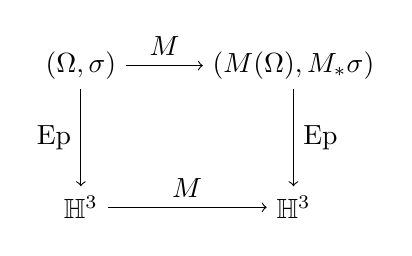
\begin{tikzpicture}[scale=0.9]
\node (1) at (0,2) {$(\Omega,\sigma)$};
\node (2) at (3,2) {$(M(\Omega),M_*\sigma)$};
\node (3) at (0,0) {$\H^3$};
\node (4) at (3,0) {$\H^3$};


\draw[->] (1) to node [above] {$M$} (2);
\draw[->] (1) to node [left] {$\mathrm{Ep}$} (3);
\draw[->] (3) to node [above] {$M$} (4);
\draw[->] (2) to node [right] {$\mathrm{Ep}$} (4);
\end{tikzpicture}
\]
That is, $\mathrm{Ep}_{M_*\sigma}(M(z)) = M( \mathrm{Ep}_{\sigma}(z))$. 
This is because both $M \circ \mathrm{Ep}_\sigma$ and $\mathrm{Ep}_{M_*\sigma} \circ M$ as maps on $\Omega$ satisfy the visual metric condition from Theorem \ref{epstein-map-def} (see \cite{anderson1998} for more details ).

This allows us to define Epstein maps on certain quotients. 
Suppose in general that $\Gamma$ is a subgroup of $\mathrm{SL}_2\C$ acting freely and properly discontinuously on $\H^3 \cup \CP^1$ leaving a domain $\Omega$ invariant. 
Then $\Omega/\Gamma$ inherits a Riemann surface structure. 
Call this structure $X$ and let $\sigma$ be a conformal metric  on $X$.
Lift this to $\tilde{\sigma}$ on $\Omega$, which is $\Gamma$-invariant. 
Then $\mathrm{Ep}_{\tilde{\sigma}}: \Omega \to \H^3$ is $\Gamma$-equivariant and therefore descends to a map $\mathrm{Ep}_\sigma : X \to \H^3/ \Gamma$. 
In particular, when $\Gamma$ is a quasi-Fuchsian group and $\Omega$ a component of the domain of discontinuity, each conformal metric $\sigma$ on the surface at infinity $X$ gives rise to a map from $X$ into the quasi-Fuchsian manifold $M$.

Uniqueness also shows us that the surfaces parallel to an Epstein surface are themselves Epstein surfaces. 
More specifically, let $g^t : U \H^3 \to \H^3$ denote the time-$t$ geodesic flow projected down to $\H^3$.
Thus for a unit tangent vector $v$ on $\H^3$ we have $g^t(v) = \exp_p(tv)$.
Using the lift of an Epstein surface to $U\H^3$ described above, each Epstein surface gives rise to a family of surfaces by applying the geodesic flow (and projecting to $\H^3$). 
That is, we have the flowed surfaces $g^t \circ \widehat{\mathrm{Ep}}_\sigma(\Omega)$. 
These surfaces are themselves Epstein surfaces corresponding to scalar multiples of $\sigma$. 
Indeed, since the parallel flow of a horosphere is a horosphere, we know $[g^t(\widehat{\mathrm{Ep}}_\sigma(z)),z] = [\mathrm{Ep}_\sigma(z),z] + t$. 
This shows us
\[
V_{g^t(\widehat{\mathrm{Ep}}_\sigma(z))}(z) = e^{2[g^t(\widehat{\mathrm{Ep}}_\sigma(z)),z]}\overset{\circ}{\sigma}(z) = e^{2t}e^{2[\mathrm{Ep}_\sigma(z),z]}\overset{\circ}{\sigma}(z) = e^{2t}\sigma(z).
\]
But the unique map that satisfies this equality is $\mathrm{Ep}_{e^{2t}\sigma}$. 
In summary, we have the following lemma, attributed to Thurston (unpublished work) by Epstein in \cite{epstein1984}.
\begin{lem}
\label{epstein-flow}
Let $\Omega$ be a domain in $\CP^1$ and $\sigma$ a conformal metric on $\Omega$.
Then 
\[
g^t \circ \widehat{\mathrm{Ep}}_\sigma  = \mathrm{Ep}_{e^{2t} \sigma}.
\]
That is, flowing the Epstein surface for $\sigma$ for time $t$ in the normal direction corresponds to taking the Epstein surface for the metric $e^{2t}\sigma$.
\end{lem}

\section{Geometry of Epstein surfaces}
\label{epstein-geometry}

The first fundamental form of the Epstein surface for the metric $\sigma$ is given by $I(\sigma) = \mathrm{Ep}_\sigma^*(g_{\H^3})$ for $g_{\H^3}$ the metric of $\H^3$. 
It is given by 
\[
I(\sigma) = 4|B(g_{\CP^1},\sigma)|^2\sigma^{-1} + \frac{1}{4}(1-K(\sigma))^2\sigma + 2(1-K(\sigma))\text{Re}(B(g_{\CP^1},\sigma)).
\]
The second fundamental form (relative to the normal lift $\widehat{\mathrm{Ep}}_\sigma$) is 
\[
\two(\sigma)
= 4|B(g_{\CP^1},\sigma)|^2\sigma^{-1} - \frac{1}{4} (1 - K(\sigma)^2)\sigma - 2 K(\sigma) \text{Re}(B(g_{\CP^1},\sigma)).
\]
These formulas are derived in \cite[Eqns.~3.2-3.3]{dumas2017}.
Here $K(\sigma)$ is the Gaussian curvature of $\sigma$ and $B(g_{\CP^1},\sigma)$ the Schwarzian derivative of $\sigma$ with respect to a M\"obius flat metric. 
We note that when the Epstein surface is embedded, its second fundamental form is negative definite due to our convenient choice of normal vector field.
Writing $\det(g)$ for the determinant of the matrix representation of $g$ relative to some local frame for the tangent bundle, the metrics on $\sigma$ and $I(\sigma)$ on $S$ have determinants related by
\[
\det(I(\sigma)) = \left( (1-K(\sigma))^2 - 16 |B(g_{\CP^1},\sigma)|^2\sigma^{-2} \right)^2 \det(\sigma).
\]
This equation is independent of the frame and has in intrinsic meaning, namely it describes the ratio of volume forms of these two metrics. 
We can compute the Gaussian curvature by $K(I(\sigma)) = -1 + \det(I(\sigma)^{-1}\two(\sigma))$ and the mean curvature by $H(\mathrm{Ep}_\sigma) = \frac{1}{2}\mathrm{tr}(I(\sigma)^{-1}\two(\sigma))$. 
We obtain
\[
K(I(\sigma))
= \frac{4K(\sigma)}{(1-K(\sigma))^2 - 16|B(g_{\CP^1},\sigma)|^2\sigma^{-2}}
\]
and
\[
H(\mathrm{Ep}_\sigma)
= \frac{K(\sigma)^2 - 1 - 16 |B(g_{\CP^1},\sigma)|^2\sigma^{-2}}{(K(\sigma) - 1)^2 - 16 |B(g_{\CP^1},\sigma)|^2\sigma^{-2}}.
\]

 
In the quasi-Fuchsian setting, if $\sigma$ is a $\Gamma$-invariant conformal metric on $\Omega$ then each term in the above equations is also $\Gamma$-invariant. 
This may be less clear for the quadratic differential $B(g_{\CP^1},\sigma)$ since the M\"obius flat metric $g_{\CP^1}$ is not itself $\Gamma$-invariant. 
However, we see that for $\gamma \in \Gamma$ we have $\gamma^*B(g_{\CP^1},\sigma) = B(\gamma^*g_{\CP^1},\gamma^*\sigma) = B(\gamma^* g_{\CP^1},\sigma)$, by naturality of Schwarzian derivatives of conformal metrics. 
The metric $\gamma^* g_{\CP^1}$ is still a M\"obius flat metric, and so $B(\gamma^* g_{\CP^1},\sigma) = B(g_{\CP^1},\sigma)$, implying $B(g_{\CP^1}, \sigma)$ is $\Gamma$-invariant. 
Therefore, $B(g_{\CP^1},\sigma)$ induces a quadratic differential on $X$, which we will denote by $B(\sigma)$.

In summary of the above, we have the following Gaussian and mean curvatures of the Epstein surfaces in $M$.
\begin{lem}
\label{curvature-epstein}
The Gaussian curvature for the Epstein surface $\mathrm{Ep}_\sigma : X \to M$ is given by
\[
K(I(\sigma))
= \frac{4K(\sigma)}{(1-K(\sigma))^2 - 16 |B(g_{\CP^1},\sigma)|^2\sigma^{-2}},
\]
and the mean curvature by 
\[
\pushQED{\qed}
H(\mathrm{Ep}_\sigma)
= \frac{K(\sigma)^2 - 1 - 16 |B(g_{\CP^1},\sigma)|^2\sigma^{-2}}{(K(\sigma) - 1)^2 - 16 |B(g_{\CP^1},\sigma)|^2\sigma^{-2}}.
\qedhere
\popQED
\]
\end{lem}
These are now equations on the compact Riemann surface $X$.

\chapter{Epstein Surfaces}
\label{epstein-surfaces}

\section{The visual metric construction}


A natural trivialization of the unit tangent bundle of hyperbolic space $U\H^3$ is given as
\[
U\H^3 \to \H^3 \times \CP^1
\quad \text{ by } \quad
(p,v) \mapsto (p, \lim_{t \to \infty} \exp_p (tv) ).
\]
That is we map $(p,v)$ to the ideal endpoint of the geodesic ray through $p$ in the direction $v$. 
Restricting to a point $p$ and using the diffeomorphism $U_p\H^3 \to \CP^1$, we can push forward to $\CP^1$ the induced metric on $U_p\H^3$ considered as a submanifold of $T_p\H^3$ with metric given by the inner product $g_{\H^3}(p)$. 
The resulting metric $V_p$ on $\CP^1$ is called the visual metric from $p$.
As an example, the visual metric from the origin in the ball model $V_0$ is just the spherical metric $\overset{\circ}{\sigma}$ on $S^2$ (which is identified with $\CP^1$ in this model). 
In general, if $M \in \mathrm{PSL}_2\C$ is an isometry taking $0$ to the point $p$, then $V_p = M_*V_0$. 

As the spherical metric belongs to the conformal class of $\CP^1$, we have that $V_0$ is a conformal metric. 
Since M\"obius transformations are biholomorphisms of $\CP^1$, each $V_p$ is also a conformal metric. 
If we work in the ball model of hyperbolic space $\H^3 \cong \mathbb{B}^3$ we can actually be explicit regarding the conformal factor between $V_p$ and $\overset{\circ}{\sigma}$ using the affine parameter of a horosphere. 
If $H$ is a horosphere, then its affine parameter is the signed hyperbolic distance from $0 \in \H^3$ to $H$, positive if $0$ is outside $H$ and negative if inside. 
Then for $p \in \H^3$ there is a unique horosphere based at $z \in \CP^1$ that contains $p$. 
Denote by $[p,z]$ the affine parameter of this horosphere. 
Then
\[
V_p(z) = e^{2[p,z]}\overset{\circ}{\sigma}(z).
\]

We now describe the Visual Metric Construction (see \cite{anderson1998}). 
This is a process that, given a strictly convex surface $S$ in $\H^3$, gives a domain $\Omega$ in $\CP^1$ and a conformal metric $\sigma$ on $\Omega$.
The idea is this: Given $S$, we have its image under the Gauss map on $\CP^1$. 
That is, given a unit normal vector field $n$ on $S$ for which $S$ is strictly convex, define
\[
\mathcal{G}:S \to \CP^1 \text{ by } \mathcal{G}(p) = \lim_{t \to \infty} \exp_p(t n(p)).
\]
The strict convexity of $S$ guarantees the map $\mathcal{G}$ is a local homeomorphism. 
We assume now that it is actually a homeomorphism.
The image surface also comes equipped with a metric $\sigma$ by defining $\sigma(\mathcal{G}(p)) = V_p(\mathcal{G}(p))$. 
Since for each $p$ the visual metric from $p$ is a conformal metric on $\CP^1$, we have $\sigma$ itself is a conformal metric. 

Epstein in \cite{epstein1984} describes an inverse process to the visual metric construction, which we describe below.

\section{The Epstein map}


As an inverse to the visual metric construction above, the Epstein map takes a domain $\Omega$ in $\CP^1$ and a conformal metric $\sigma$ on $\Omega$ and describes a strictly convex surface $f: \Omega \to \H^3$. 
This surface has the property that $V_{f(z)}(z) = \sigma(z)$ and this property can be used to derive a formula for the surface. 
Specifically, expanding upon this last condition and using the affine parameter discussed above, we see that 
\[
\sigma(z) = V_{f(z)}(z) = e^{2 [f(z),z]} \overset{\circ}{\sigma}(z),
\]
or that $f(z)$ lies on the horosphere based at $z$ with affine parameter
\[
[f(z),z] = \frac{1}{2} \log \left( \frac{\sigma(z)}{\overset{\circ}{\sigma}(z)} \right) =: \rho(z).
\]
Hence, we know which horosphere based at $z$ that $f(z)$ must lie on. 

There is a convenient choice of normal vector field. 
At $f(z)$, the geodesic in the direction $n(f(z))$ must end at $z$ in order for $f$ to be an inverse to the visual metric construction. 
The normal vectors to a horosphere pointing to its base have this property, so we define $n(f(z))$ to be the normal vector to the horosphere based at $z$ with affine parameter $\rho(z)$. 
Since $n$ must be normal to the image surface $S = f(\Omega)$, this identifies the tangent spaces to the sought-after $S$ with the tangent spaces to the horospheres. 
And this identifies the surface $S$ with the envelope of the family of horospheres
\[
\mathcal{H}(\Omega,\sigma) = \{ \text{Horosphere based at $z$ with parameter $\rho(z)$} \ | \ z \in \Omega \}.
\]


In \cite{epstein1984}, Epstein derives an equation for such an envelope. 
Working in the ball model and taking $z$ both as a point in $\CP^1 \cong S^2$ as well as a unit vector in $\R^3$, he shows the desired map is 
\[
\mathrm{Ep}_\sigma(z) = \frac{|\overset{\circ}{\nabla}\rho(z)|^2 + e^{2\rho(z)} - 1}{|\overset{\circ}{\nabla}\rho(z)|^2 + (e^{\rho(z)}+1)^2} z + \frac{2}{|\overset{\circ}{\nabla}\rho(z)|^2 + (e^{\rho(z)}+1)^2} \overset{\circ}{\nabla}\rho(z),
\]
where $\overset{\circ}{\nabla}\rho$ is the gradient of $\rho$ with respect to the spherical metric on $S^2$. 
This construction leads to the following theorem. 


\begin{thm}[Epstein \cite{epstein1984}]
Let $\Omega$ be a domain in $\CP^1$  and $\sigma$ a $C^k$ conformal metric on $\Omega$, then there exists a unique $C^{k-1}$ map $\mathrm{Ep}_\sigma : \Omega \to \H^3$, called the Epstein map of $\Omega$ for the metric $\sigma$, such that for all $z \in \Omega$,
\[
V_{\mathrm{Ep}_\sigma(z)}(z) = \sigma(z).
\]
Moreover, the image of a point $z$ depends only on the 1-jet of $\sigma$ at $z$.
\label{epstein-map-def}
\end{thm}

Epstein's original construction uses the ball model of hyperbolic space to define the Epstein map. 
In \cite{dumas2017}, Dumas gives a model independent definition of the map using an $\text{SL}_2\C$-frame field. 
It proceeds as follows. 
Choose an affine coordinate chart $z$ on $\CP^1$ that distinguishes a point $0 \in \Omega$ and $\infty \notin \Omega$. 
Then, on the geodesic in $\H^3$ with ideal endpoints $0$ and $\infty$, there exists a unique point $p$ such that the visual metric from $p$ at $0$ is the Euclidean metric of this affine chart, $V_p(0) = |dz|^2$. 
The Epstein map is an $\mathrm{SL}_2\C$-frame orbit of this point.     


\begin{prop}[\cite{dumas2017}]
On a domain $\Omega$ in $\CP^1$ write $\sigma = e^{2\eta}|dz|^2$. Define the $\mathrm{SL}_2,\C$-frame field $\widetilde{\mathrm{Ep}}_\sigma: \Omega \to \mathrm{SL}_2\C$ by 
\[
\widetilde{\mathrm{Ep}}_\sigma(z) =
\begin{pmatrix}
1 & z \\
0 & 1
\end{pmatrix}
\begin{pmatrix}
1 & 0 \\
\eta_z & 1
\end{pmatrix}
\begin{pmatrix}
e^{-\eta/2} & 0 \\
0 & e^{\eta/2}
\end{pmatrix},
\]
then the Epstein map is given by 
\[
\mathrm{Ep}_\sigma(z) = \widetilde{\mathrm{Ep}}_\sigma(z) \cdot p.
\]
\end{prop}

 

Even though we call the image an Epstein surface, the Epstein map need not be an immersion. 
Indeed, if $\sigma$ is itself a visual metric then the Epstein map for $\sigma$ is constant. 
However, the lift of $\mathrm{Ep}_\sigma$ from $\Omega$ to the unit tangent bundle of hyperbolic space given by 
\[
\widehat{\mathrm{Ep}}_\sigma(z) = (\text{Ep}_\sigma(z),z) 
\] 
is an immersion (here we are using the trivialization $U\H^3 \cong \H^3 \times \CP^1$ defined above). 
This lift can be thought of as providing a unit ``normal'' vector field for the Epstein surface even when the Epstein map is not an immersion. 
Indeed, this lift agrees with a unit normal vector field when the surface is immersed and so we will simply refer to it as the normal field from now on. 

Because the Epstein map is unique, it is natural with respect to the action of $\mathrm{SL}_2\C$ in the following sense. 
Suppose $M \in \mathrm{SL}_2\C$, then the following diagram commutes:
\[
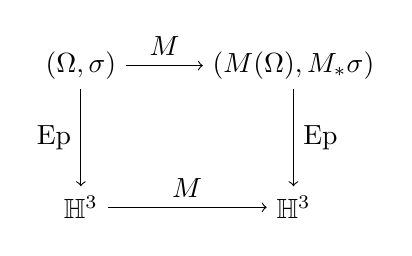
\begin{tikzpicture}[scale=0.9]
\node (1) at (0,2) {$(\Omega,\sigma)$};
\node (2) at (3,2) {$(M(\Omega),M_*\sigma)$};
\node (3) at (0,0) {$\H^3$};
\node (4) at (3,0) {$\H^3$};


\draw[->] (1) to node [above] {$M$} (2);
\draw[->] (1) to node [left] {$\mathrm{Ep}$} (3);
\draw[->] (3) to node [above] {$M$} (4);
\draw[->] (2) to node [right] {$\mathrm{Ep}$} (4);
\end{tikzpicture}
\]
That is, $\mathrm{Ep}_{M_*\sigma}(M(z)) = M( \mathrm{Ep}_{\sigma}(z))$. 
This is because both $M \circ \mathrm{Ep}_\sigma$ and $\mathrm{Ep}_{M_*\sigma} \circ M$ as maps on $\Omega$ satisfy the visual metric condition from Theorem \ref{epstein-map-def} (see \cite{anderson1998} for more details ).

This allows us to define Epstein maps on certain quotients. 
Suppose in general that $\Gamma$ is a subgroup of $\mathrm{SL}_2\C$ acting freely and properly discontinuously on $\H^3 \cup \CP^1$ leaving a domain $\Omega$ invariant. 
Then $\Omega/\Gamma$ inherits a Riemann surface structure. 
Call this structure $X$ and let $\sigma$ be a conformal metric  on $X$.
Lift this to $\tilde{\sigma}$ on $\Omega$, which is $\Gamma$-invariant. 
Then $\mathrm{Ep}_{\tilde{\sigma}}: \Omega \to \H^3$ is $\Gamma$-equivariant and therefore descends to a map $\mathrm{Ep}_\sigma : X \to \H^3/ \Gamma$. 
In particular, when $\Gamma$ is a quasi-Fuchsian group and $\Omega$ a component of the domain of discontinuity, each conformal metric $\sigma$ on the surface at infinity $X$ gives rise to a map from $X$ into the quasi-Fuchsian manifold $M$.

Uniqueness also shows us that the surfaces parallel to an Epstein surface are themselves Epstein surfaces. 
More specifically, let $g^t : U \H^3 \to \H^3$ denote the time-$t$ geodesic flow projected down to $\H^3$.
Thus for a unit tangent vector $v$ on $\H^3$ we have $g^t(v) = \exp_p(tv)$.
Using the lift of an Epstein surface to $U\H^3$ described above, each Epstein surface gives rise to a family of surfaces by applying the geodesic flow (and projecting to $\H^3$). 
That is, we have the flowed surfaces $g^t \circ \widehat{\mathrm{Ep}}_\sigma(\Omega)$. 
These surfaces are themselves Epstein surfaces corresponding to scalar multiples of $\sigma$. 
Indeed, since the parallel flow of a horosphere is a horosphere, we know $[g^t(\widehat{\mathrm{Ep}}_\sigma(z)),z] = [\mathrm{Ep}_\sigma(z),z] + t$. 
This shows us
\[
V_{g^t(\widehat{\mathrm{Ep}}_\sigma(z))}(z) = e^{2[g^t(\widehat{\mathrm{Ep}}_\sigma(z)),z]}\overset{\circ}{\sigma}(z) = e^{2t}e^{2[\mathrm{Ep}_\sigma(z),z]}\overset{\circ}{\sigma}(z) = e^{2t}\sigma(z).
\]
But the unique map that satisfies this equality is $\mathrm{Ep}_{e^{2t}\sigma}$. 
In summary, we have the following lemma, attributed to Thurston (unpublished work) by Epstein in \cite{epstein1984}.
\begin{lem}
\label{epstein-flow}
Let $\Omega$ be a domain in $\CP^1$ and $\sigma$ a conformal metric on $\Omega$.
Then 
\[
g^t \circ \widehat{\mathrm{Ep}}_\sigma  = \mathrm{Ep}_{e^{2t} \sigma}.
\]
That is, flowing the Epstein surface for $\sigma$ for time $t$ in the normal direction corresponds to taking the Epstein surface for the metric $e^{2t}\sigma$.
\end{lem}

\section{Geometry of Epstein surfaces}
\label{epstein-geometry}

The first fundamental form of the Epstein surface for the metric $\sigma$ is given by $I(\sigma) = \mathrm{Ep}_\sigma^*(g_{\H^3})$ for $g_{\H^3}$ the metric of $\H^3$. 
It is given by 
\[
I(\sigma) = 4|B(g_{\CP^1},\sigma)|^2\sigma^{-1} + \frac{1}{4}(1-K(\sigma))^2\sigma + 2(1-K(\sigma))\text{Re}(B(g_{\CP^1},\sigma)).
\]
The second fundamental form (relative to the normal lift $\widehat{\mathrm{Ep}}_\sigma$) is 
\[
\two(\sigma)
= 4|B(g_{\CP^1},\sigma)|^2\sigma^{-1} - \frac{1}{4} (1 - K(\sigma)^2)\sigma - 2 K(\sigma) \text{Re}(B(g_{\CP^1},\sigma)).
\]
These formulas are derived in \cite[Eqns.~3.2-3.3]{dumas2017}.
Here $K(\sigma)$ is the Gaussian curvature of $\sigma$ and $B(g_{\CP^1},\sigma)$ the Schwarzian derivative of $\sigma$ with respect to a M\"obius flat metric. 
We note that when the Epstein surface is embedded, its second fundamental form is negative definite due to our convenient choice of normal vector field.
Writing $\det(g)$ for the determinant of the matrix representation of $g$ relative to some local frame for the tangent bundle, the metrics on $\sigma$ and $I(\sigma)$ on $S$ have determinants related by
\[
\det(I(\sigma)) = \left( (1-K(\sigma))^2 - 16 |B(g_{\CP^1},\sigma)|^2\sigma^{-2} \right)^2 \det(\sigma).
\]
This equation is independent of the frame and has in intrinsic meaning, namely it describes the ratio of volume forms of these two metrics. 
We can compute the Gaussian curvature by $K(I(\sigma)) = -1 + \det(I(\sigma)^{-1}\two(\sigma))$ and the mean curvature by $H(\mathrm{Ep}_\sigma) = \frac{1}{2}\mathrm{tr}(I(\sigma)^{-1}\two(\sigma))$. 
We obtain
\[
K(I(\sigma))
= \frac{4K(\sigma)}{(1-K(\sigma))^2 - 16|B(g_{\CP^1},\sigma)|^2\sigma^{-2}}
\]
and
\[
H(\mathrm{Ep}_\sigma)
= \frac{K(\sigma)^2 - 1 - 16 |B(g_{\CP^1},\sigma)|^2\sigma^{-2}}{(K(\sigma) - 1)^2 - 16 |B(g_{\CP^1},\sigma)|^2\sigma^{-2}}.
\]

 
In the quasi-Fuchsian setting, if $\sigma$ is a $\Gamma$-invariant conformal metric on $\Omega$ then each term in the above equations is also $\Gamma$-invariant. 
This may be less clear for the quadratic differential $B(g_{\CP^1},\sigma)$ since the M\"obius flat metric $g_{\CP^1}$ is not itself $\Gamma$-invariant. 
However, we see that for $\gamma \in \Gamma$ we have $\gamma^*B(g_{\CP^1},\sigma) = B(\gamma^*g_{\CP^1},\gamma^*\sigma) = B(\gamma^* g_{\CP^1},\sigma)$, by naturality of Schwarzian derivatives of conformal metrics. 
The metric $\gamma^* g_{\CP^1}$ is still a M\"obius flat metric, and so $B(\gamma^* g_{\CP^1},\sigma) = B(g_{\CP^1},\sigma)$, implying $B(g_{\CP^1}, \sigma)$ is $\Gamma$-invariant. 
Therefore, $B(g_{\CP^1},\sigma)$ induces a quadratic differential on $X$, which we will denote by $B(\sigma)$.

In summary of the above, we have the following Gaussian and mean curvatures of the Epstein surfaces in $M$.
\begin{lem}
\label{curvature-epstein}
The Gaussian curvature for the Epstein surface $\mathrm{Ep}_\sigma : X \to M$ is given by
\[
K(I(\sigma))
= \frac{4K(\sigma)}{(1-K(\sigma))^2 - 16 |B(g_{\CP^1},\sigma)|^2\sigma^{-2}},
\]
and the mean curvature by 
\[
\pushQED{\qed}
H(\mathrm{Ep}_\sigma)
= \frac{K(\sigma)^2 - 1 - 16 |B(g_{\CP^1},\sigma)|^2\sigma^{-2}}{(K(\sigma) - 1)^2 - 16 |B(g_{\CP^1},\sigma)|^2\sigma^{-2}}.
\qedhere
\popQED
\]
\end{lem}
These are now equations on the compact Riemann surface $X$.

\chapter{Epstein Surfaces}
\label{epstein-surfaces}

\section{The visual metric construction}


A natural trivialization of the unit tangent bundle of hyperbolic space $U\H^3$ is given as
\[
U\H^3 \to \H^3 \times \CP^1
\quad \text{ by } \quad
(p,v) \mapsto (p, \lim_{t \to \infty} \exp_p (tv) ).
\]
That is we map $(p,v)$ to the ideal endpoint of the geodesic ray through $p$ in the direction $v$. 
Restricting to a point $p$ and using the diffeomorphism $U_p\H^3 \to \CP^1$, we can push forward to $\CP^1$ the induced metric on $U_p\H^3$ considered as a submanifold of $T_p\H^3$ with metric given by the inner product $g_{\H^3}(p)$. 
The resulting metric $V_p$ on $\CP^1$ is called the visual metric from $p$.
As an example, the visual metric from the origin in the ball model $V_0$ is just the spherical metric $\overset{\circ}{\sigma}$ on $S^2$ (which is identified with $\CP^1$ in this model). 
In general, if $M \in \mathrm{PSL}_2\C$ is an isometry taking $0$ to the point $p$, then $V_p = M_*V_0$. 

As the spherical metric belongs to the conformal class of $\CP^1$, we have that $V_0$ is a conformal metric. 
Since M\"obius transformations are biholomorphisms of $\CP^1$, each $V_p$ is also a conformal metric. 
If we work in the ball model of hyperbolic space $\H^3 \cong \mathbb{B}^3$ we can actually be explicit regarding the conformal factor between $V_p$ and $\overset{\circ}{\sigma}$ using the affine parameter of a horosphere. 
If $H$ is a horosphere, then its affine parameter is the signed hyperbolic distance from $0 \in \H^3$ to $H$, positive if $0$ is outside $H$ and negative if inside. 
Then for $p \in \H^3$ there is a unique horosphere based at $z \in \CP^1$ that contains $p$. 
Denote by $[p,z]$ the affine parameter of this horosphere. 
Then
\[
V_p(z) = e^{2[p,z]}\overset{\circ}{\sigma}(z).
\]

We now describe the Visual Metric Construction (see \cite{anderson1998}). 
This is a process that, given a strictly convex surface $S$ in $\H^3$, gives a domain $\Omega$ in $\CP^1$ and a conformal metric $\sigma$ on $\Omega$.
The idea is this: Given $S$, we have its image under the Gauss map on $\CP^1$. 
That is, given a unit normal vector field $n$ on $S$ for which $S$ is strictly convex, define
\[
\mathcal{G}:S \to \CP^1 \text{ by } \mathcal{G}(p) = \lim_{t \to \infty} \exp_p(t n(p)).
\]
The strict convexity of $S$ guarantees the map $\mathcal{G}$ is a local homeomorphism. 
We assume now that it is actually a homeomorphism.
The image surface also comes equipped with a metric $\sigma$ by defining $\sigma(\mathcal{G}(p)) = V_p(\mathcal{G}(p))$. 
Since for each $p$ the visual metric from $p$ is a conformal metric on $\CP^1$, we have $\sigma$ itself is a conformal metric. 

Epstein in \cite{epstein1984} describes an inverse process to the visual metric construction, which we describe below.

\section{The Epstein map}


As an inverse to the visual metric construction above, the Epstein map takes a domain $\Omega$ in $\CP^1$ and a conformal metric $\sigma$ on $\Omega$ and describes a strictly convex surface $f: \Omega \to \H^3$. 
This surface has the property that $V_{f(z)}(z) = \sigma(z)$ and this property can be used to derive a formula for the surface. 
Specifically, expanding upon this last condition and using the affine parameter discussed above, we see that 
\[
\sigma(z) = V_{f(z)}(z) = e^{2 [f(z),z]} \overset{\circ}{\sigma}(z),
\]
or that $f(z)$ lies on the horosphere based at $z$ with affine parameter
\[
[f(z),z] = \frac{1}{2} \log \left( \frac{\sigma(z)}{\overset{\circ}{\sigma}(z)} \right) =: \rho(z).
\]
Hence, we know which horosphere based at $z$ that $f(z)$ must lie on. 

There is a convenient choice of normal vector field. 
At $f(z)$, the geodesic in the direction $n(f(z))$ must end at $z$ in order for $f$ to be an inverse to the visual metric construction. 
The normal vectors to a horosphere pointing to its base have this property, so we define $n(f(z))$ to be the normal vector to the horosphere based at $z$ with affine parameter $\rho(z)$. 
Since $n$ must be normal to the image surface $S = f(\Omega)$, this identifies the tangent spaces to the sought-after $S$ with the tangent spaces to the horospheres. 
And this identifies the surface $S$ with the envelope of the family of horospheres
\[
\mathcal{H}(\Omega,\sigma) = \{ \text{Horosphere based at $z$ with parameter $\rho(z)$} \ | \ z \in \Omega \}.
\]


In \cite{epstein1984}, Epstein derives an equation for such an envelope. 
Working in the ball model and taking $z$ both as a point in $\CP^1 \cong S^2$ as well as a unit vector in $\R^3$, he shows the desired map is 
\[
\mathrm{Ep}_\sigma(z) = \frac{|\overset{\circ}{\nabla}\rho(z)|^2 + e^{2\rho(z)} - 1}{|\overset{\circ}{\nabla}\rho(z)|^2 + (e^{\rho(z)}+1)^2} z + \frac{2}{|\overset{\circ}{\nabla}\rho(z)|^2 + (e^{\rho(z)}+1)^2} \overset{\circ}{\nabla}\rho(z),
\]
where $\overset{\circ}{\nabla}\rho$ is the gradient of $\rho$ with respect to the spherical metric on $S^2$. 
This construction leads to the following theorem. 


\begin{thm}[Epstein \cite{epstein1984}]
Let $\Omega$ be a domain in $\CP^1$  and $\sigma$ a $C^k$ conformal metric on $\Omega$, then there exists a unique $C^{k-1}$ map $\mathrm{Ep}_\sigma : \Omega \to \H^3$, called the Epstein map of $\Omega$ for the metric $\sigma$, such that for all $z \in \Omega$,
\[
V_{\mathrm{Ep}_\sigma(z)}(z) = \sigma(z).
\]
Moreover, the image of a point $z$ depends only on the 1-jet of $\sigma$ at $z$.
\label{epstein-map-def}
\end{thm}

Epstein's original construction uses the ball model of hyperbolic space to define the Epstein map. 
In \cite{dumas2017}, Dumas gives a model independent definition of the map using an $\text{SL}_2\C$-frame field. 
It proceeds as follows. 
Choose an affine coordinate chart $z$ on $\CP^1$ that distinguishes a point $0 \in \Omega$ and $\infty \notin \Omega$. 
Then, on the geodesic in $\H^3$ with ideal endpoints $0$ and $\infty$, there exists a unique point $p$ such that the visual metric from $p$ at $0$ is the Euclidean metric of this affine chart, $V_p(0) = |dz|^2$. 
The Epstein map is an $\mathrm{SL}_2\C$-frame orbit of this point.     


\begin{prop}[\cite{dumas2017}]
On a domain $\Omega$ in $\CP^1$ write $\sigma = e^{2\eta}|dz|^2$. Define the $\mathrm{SL}_2,\C$-frame field $\widetilde{\mathrm{Ep}}_\sigma: \Omega \to \mathrm{SL}_2\C$ by 
\[
\widetilde{\mathrm{Ep}}_\sigma(z) =
\begin{pmatrix}
1 & z \\
0 & 1
\end{pmatrix}
\begin{pmatrix}
1 & 0 \\
\eta_z & 1
\end{pmatrix}
\begin{pmatrix}
e^{-\eta/2} & 0 \\
0 & e^{\eta/2}
\end{pmatrix},
\]
then the Epstein map is given by 
\[
\mathrm{Ep}_\sigma(z) = \widetilde{\mathrm{Ep}}_\sigma(z) \cdot p.
\]
\end{prop}

 

Even though we call the image an Epstein surface, the Epstein map need not be an immersion. 
Indeed, if $\sigma$ is itself a visual metric then the Epstein map for $\sigma$ is constant. 
However, the lift of $\mathrm{Ep}_\sigma$ from $\Omega$ to the unit tangent bundle of hyperbolic space given by 
\[
\widehat{\mathrm{Ep}}_\sigma(z) = (\text{Ep}_\sigma(z),z) 
\] 
is an immersion (here we are using the trivialization $U\H^3 \cong \H^3 \times \CP^1$ defined above). 
This lift can be thought of as providing a unit ``normal'' vector field for the Epstein surface even when the Epstein map is not an immersion. 
Indeed, this lift agrees with a unit normal vector field when the surface is immersed and so we will simply refer to it as the normal field from now on. 

Because the Epstein map is unique, it is natural with respect to the action of $\mathrm{SL}_2\C$ in the following sense. 
Suppose $M \in \mathrm{SL}_2\C$, then the following diagram commutes:
\[
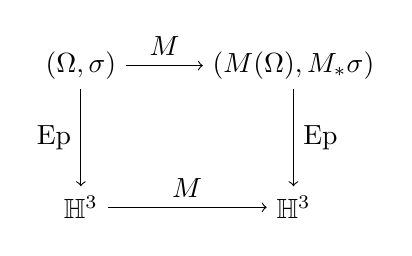
\begin{tikzpicture}[scale=0.9]
\node (1) at (0,2) {$(\Omega,\sigma)$};
\node (2) at (3,2) {$(M(\Omega),M_*\sigma)$};
\node (3) at (0,0) {$\H^3$};
\node (4) at (3,0) {$\H^3$};


\draw[->] (1) to node [above] {$M$} (2);
\draw[->] (1) to node [left] {$\mathrm{Ep}$} (3);
\draw[->] (3) to node [above] {$M$} (4);
\draw[->] (2) to node [right] {$\mathrm{Ep}$} (4);
\end{tikzpicture}
\]
That is, $\mathrm{Ep}_{M_*\sigma}(M(z)) = M( \mathrm{Ep}_{\sigma}(z))$. 
This is because both $M \circ \mathrm{Ep}_\sigma$ and $\mathrm{Ep}_{M_*\sigma} \circ M$ as maps on $\Omega$ satisfy the visual metric condition from Theorem \ref{epstein-map-def} (see \cite{anderson1998} for more details ).

This allows us to define Epstein maps on certain quotients. 
Suppose in general that $\Gamma$ is a subgroup of $\mathrm{SL}_2\C$ acting freely and properly discontinuously on $\H^3 \cup \CP^1$ leaving a domain $\Omega$ invariant. 
Then $\Omega/\Gamma$ inherits a Riemann surface structure. 
Call this structure $X$ and let $\sigma$ be a conformal metric  on $X$.
Lift this to $\tilde{\sigma}$ on $\Omega$, which is $\Gamma$-invariant. 
Then $\mathrm{Ep}_{\tilde{\sigma}}: \Omega \to \H^3$ is $\Gamma$-equivariant and therefore descends to a map $\mathrm{Ep}_\sigma : X \to \H^3/ \Gamma$. 
In particular, when $\Gamma$ is a quasi-Fuchsian group and $\Omega$ a component of the domain of discontinuity, each conformal metric $\sigma$ on the surface at infinity $X$ gives rise to a map from $X$ into the quasi-Fuchsian manifold $M$.

Uniqueness also shows us that the surfaces parallel to an Epstein surface are themselves Epstein surfaces. 
More specifically, let $g^t : U \H^3 \to \H^3$ denote the time-$t$ geodesic flow projected down to $\H^3$.
Thus for a unit tangent vector $v$ on $\H^3$ we have $g^t(v) = \exp_p(tv)$.
Using the lift of an Epstein surface to $U\H^3$ described above, each Epstein surface gives rise to a family of surfaces by applying the geodesic flow (and projecting to $\H^3$). 
That is, we have the flowed surfaces $g^t \circ \widehat{\mathrm{Ep}}_\sigma(\Omega)$. 
These surfaces are themselves Epstein surfaces corresponding to scalar multiples of $\sigma$. 
Indeed, since the parallel flow of a horosphere is a horosphere, we know $[g^t(\widehat{\mathrm{Ep}}_\sigma(z)),z] = [\mathrm{Ep}_\sigma(z),z] + t$. 
This shows us
\[
V_{g^t(\widehat{\mathrm{Ep}}_\sigma(z))}(z) = e^{2[g^t(\widehat{\mathrm{Ep}}_\sigma(z)),z]}\overset{\circ}{\sigma}(z) = e^{2t}e^{2[\mathrm{Ep}_\sigma(z),z]}\overset{\circ}{\sigma}(z) = e^{2t}\sigma(z).
\]
But the unique map that satisfies this equality is $\mathrm{Ep}_{e^{2t}\sigma}$. 
In summary, we have the following lemma, attributed to Thurston (unpublished work) by Epstein in \cite{epstein1984}.
\begin{lem}
\label{epstein-flow}
Let $\Omega$ be a domain in $\CP^1$ and $\sigma$ a conformal metric on $\Omega$.
Then 
\[
g^t \circ \widehat{\mathrm{Ep}}_\sigma  = \mathrm{Ep}_{e^{2t} \sigma}.
\]
That is, flowing the Epstein surface for $\sigma$ for time $t$ in the normal direction corresponds to taking the Epstein surface for the metric $e^{2t}\sigma$.
\end{lem}

\section{Geometry of Epstein surfaces}
\label{epstein-geometry}

The first fundamental form of the Epstein surface for the metric $\sigma$ is given by $I(\sigma) = \mathrm{Ep}_\sigma^*(g_{\H^3})$ for $g_{\H^3}$ the metric of $\H^3$. 
It is given by 
\[
I(\sigma) = 4|B(g_{\CP^1},\sigma)|^2\sigma^{-1} + \frac{1}{4}(1-K(\sigma))^2\sigma + 2(1-K(\sigma))\text{Re}(B(g_{\CP^1},\sigma)).
\]
The second fundamental form (relative to the normal lift $\widehat{\mathrm{Ep}}_\sigma$) is 
\[
\two(\sigma)
= 4|B(g_{\CP^1},\sigma)|^2\sigma^{-1} - \frac{1}{4} (1 - K(\sigma)^2)\sigma - 2 K(\sigma) \text{Re}(B(g_{\CP^1},\sigma)).
\]
These formulas are derived in \cite[Eqns.~3.2-3.3]{dumas2017}.
Here $K(\sigma)$ is the Gaussian curvature of $\sigma$ and $B(g_{\CP^1},\sigma)$ the Schwarzian derivative of $\sigma$ with respect to a M\"obius flat metric. 
We note that when the Epstein surface is embedded, its second fundamental form is negative definite due to our convenient choice of normal vector field.
Writing $\det(g)$ for the determinant of the matrix representation of $g$ relative to some local frame for the tangent bundle, the metrics on $\sigma$ and $I(\sigma)$ on $S$ have determinants related by
\[
\det(I(\sigma)) = \left( (1-K(\sigma))^2 - 16 |B(g_{\CP^1},\sigma)|^2\sigma^{-2} \right)^2 \det(\sigma).
\]
This equation is independent of the frame and has in intrinsic meaning, namely it describes the ratio of volume forms of these two metrics. 
We can compute the Gaussian curvature by $K(I(\sigma)) = -1 + \det(I(\sigma)^{-1}\two(\sigma))$ and the mean curvature by $H(\mathrm{Ep}_\sigma) = \frac{1}{2}\mathrm{tr}(I(\sigma)^{-1}\two(\sigma))$. 
We obtain
\[
K(I(\sigma))
= \frac{4K(\sigma)}{(1-K(\sigma))^2 - 16|B(g_{\CP^1},\sigma)|^2\sigma^{-2}}
\]
and
\[
H(\mathrm{Ep}_\sigma)
= \frac{K(\sigma)^2 - 1 - 16 |B(g_{\CP^1},\sigma)|^2\sigma^{-2}}{(K(\sigma) - 1)^2 - 16 |B(g_{\CP^1},\sigma)|^2\sigma^{-2}}.
\]

 
In the quasi-Fuchsian setting, if $\sigma$ is a $\Gamma$-invariant conformal metric on $\Omega$ then each term in the above equations is also $\Gamma$-invariant. 
This may be less clear for the quadratic differential $B(g_{\CP^1},\sigma)$ since the M\"obius flat metric $g_{\CP^1}$ is not itself $\Gamma$-invariant. 
However, we see that for $\gamma \in \Gamma$ we have $\gamma^*B(g_{\CP^1},\sigma) = B(\gamma^*g_{\CP^1},\gamma^*\sigma) = B(\gamma^* g_{\CP^1},\sigma)$, by naturality of Schwarzian derivatives of conformal metrics. 
The metric $\gamma^* g_{\CP^1}$ is still a M\"obius flat metric, and so $B(\gamma^* g_{\CP^1},\sigma) = B(g_{\CP^1},\sigma)$, implying $B(g_{\CP^1}, \sigma)$ is $\Gamma$-invariant. 
Therefore, $B(g_{\CP^1},\sigma)$ induces a quadratic differential on $X$, which we will denote by $B(\sigma)$.

In summary of the above, we have the following Gaussian and mean curvatures of the Epstein surfaces in $M$.
\begin{lem}
\label{curvature-epstein}
The Gaussian curvature for the Epstein surface $\mathrm{Ep}_\sigma : X \to M$ is given by
\[
K(I(\sigma))
= \frac{4K(\sigma)}{(1-K(\sigma))^2 - 16 |B(g_{\CP^1},\sigma)|^2\sigma^{-2}},
\]
and the mean curvature by 
\[
\pushQED{\qed}
H(\mathrm{Ep}_\sigma)
= \frac{K(\sigma)^2 - 1 - 16 |B(g_{\CP^1},\sigma)|^2\sigma^{-2}}{(K(\sigma) - 1)^2 - 16 |B(g_{\CP^1},\sigma)|^2\sigma^{-2}}.
\qedhere
\popQED
\]
\end{lem}
These are now equations on the compact Riemann surface $X$.

\chapter{Epstein Surfaces}
\label{epstein-surfaces}

\section{The visual metric construction}


A natural trivialization of the unit tangent bundle of hyperbolic space $U\H^3$ is given as
\[
U\H^3 \to \H^3 \times \CP^1
\quad \text{ by } \quad
(p,v) \mapsto (p, \lim_{t \to \infty} \exp_p (tv) ).
\]
That is we map $(p,v)$ to the ideal endpoint of the geodesic ray through $p$ in the direction $v$. 
Restricting to a point $p$ and using the diffeomorphism $U_p\H^3 \to \CP^1$, we can push forward to $\CP^1$ the induced metric on $U_p\H^3$ considered as a submanifold of $T_p\H^3$ with metric given by the inner product $g_{\H^3}(p)$. 
The resulting metric $V_p$ on $\CP^1$ is called the visual metric from $p$.
As an example, the visual metric from the origin in the ball model $V_0$ is just the spherical metric $\overset{\circ}{\sigma}$ on $S^2$ (which is identified with $\CP^1$ in this model). 
In general, if $M \in \mathrm{PSL}_2\C$ is an isometry taking $0$ to the point $p$, then $V_p = M_*V_0$. 

As the spherical metric belongs to the conformal class of $\CP^1$, we have that $V_0$ is a conformal metric. 
Since M\"obius transformations are biholomorphisms of $\CP^1$, each $V_p$ is also a conformal metric. 
If we work in the ball model of hyperbolic space $\H^3 \cong \mathbb{B}^3$ we can actually be explicit regarding the conformal factor between $V_p$ and $\overset{\circ}{\sigma}$ using the affine parameter of a horosphere. 
If $H$ is a horosphere, then its affine parameter is the signed hyperbolic distance from $0 \in \H^3$ to $H$, positive if $0$ is outside $H$ and negative if inside. 
Then for $p \in \H^3$ there is a unique horosphere based at $z \in \CP^1$ that contains $p$. 
Denote by $[p,z]$ the affine parameter of this horosphere. 
Then
\[
V_p(z) = e^{2[p,z]}\overset{\circ}{\sigma}(z).
\]

We now describe the Visual Metric Construction (see \cite{anderson1998}). 
This is a process that, given a strictly convex surface $S$ in $\H^3$, gives a domain $\Omega$ in $\CP^1$ and a conformal metric $\sigma$ on $\Omega$.
The idea is this: Given $S$, we have its image under the Gauss map on $\CP^1$. 
That is, given a unit normal vector field $n$ on $S$ for which $S$ is strictly convex, define
\[
\mathcal{G}:S \to \CP^1 \text{ by } \mathcal{G}(p) = \lim_{t \to \infty} \exp_p(t n(p)).
\]
The strict convexity of $S$ guarantees the map $\mathcal{G}$ is a local homeomorphism. 
We assume now that it is actually a homeomorphism.
The image surface also comes equipped with a metric $\sigma$ by defining $\sigma(\mathcal{G}(p)) = V_p(\mathcal{G}(p))$. 
Since for each $p$ the visual metric from $p$ is a conformal metric on $\CP^1$, we have $\sigma$ itself is a conformal metric. 

Epstein in \cite{epstein1984} describes an inverse process to the visual metric construction, which we describe below.

\section{The Epstein map}


As an inverse to the visual metric construction above, the Epstein map takes a domain $\Omega$ in $\CP^1$ and a conformal metric $\sigma$ on $\Omega$ and describes a strictly convex surface $f: \Omega \to \H^3$. 
This surface has the property that $V_{f(z)}(z) = \sigma(z)$ and this property can be used to derive a formula for the surface. 
Specifically, expanding upon this last condition and using the affine parameter discussed above, we see that 
\[
\sigma(z) = V_{f(z)}(z) = e^{2 [f(z),z]} \overset{\circ}{\sigma}(z),
\]
or that $f(z)$ lies on the horosphere based at $z$ with affine parameter
\[
[f(z),z] = \frac{1}{2} \log \left( \frac{\sigma(z)}{\overset{\circ}{\sigma}(z)} \right) =: \rho(z).
\]
Hence, we know which horosphere based at $z$ that $f(z)$ must lie on. 

There is a convenient choice of normal vector field. 
At $f(z)$, the geodesic in the direction $n(f(z))$ must end at $z$ in order for $f$ to be an inverse to the visual metric construction. 
The normal vectors to a horosphere pointing to its base have this property, so we define $n(f(z))$ to be the normal vector to the horosphere based at $z$ with affine parameter $\rho(z)$. 
Since $n$ must be normal to the image surface $S = f(\Omega)$, this identifies the tangent spaces to the sought-after $S$ with the tangent spaces to the horospheres. 
And this identifies the surface $S$ with the envelope of the family of horospheres
\[
\mathcal{H}(\Omega,\sigma) = \{ \text{Horosphere based at $z$ with parameter $\rho(z)$} \ | \ z \in \Omega \}.
\]


In \cite{epstein1984}, Epstein derives an equation for such an envelope. 
Working in the ball model and taking $z$ both as a point in $\CP^1 \cong S^2$ as well as a unit vector in $\R^3$, he shows the desired map is 
\[
\mathrm{Ep}_\sigma(z) = \frac{|\overset{\circ}{\nabla}\rho(z)|^2 + e^{2\rho(z)} - 1}{|\overset{\circ}{\nabla}\rho(z)|^2 + (e^{\rho(z)}+1)^2} z + \frac{2}{|\overset{\circ}{\nabla}\rho(z)|^2 + (e^{\rho(z)}+1)^2} \overset{\circ}{\nabla}\rho(z),
\]
where $\overset{\circ}{\nabla}\rho$ is the gradient of $\rho$ with respect to the spherical metric on $S^2$. 
This construction leads to the following theorem. 


\begin{thm}[Epstein \cite{epstein1984}]
Let $\Omega$ be a domain in $\CP^1$  and $\sigma$ a $C^k$ conformal metric on $\Omega$, then there exists a unique $C^{k-1}$ map $\mathrm{Ep}_\sigma : \Omega \to \H^3$, called the Epstein map of $\Omega$ for the metric $\sigma$, such that for all $z \in \Omega$,
\[
V_{\mathrm{Ep}_\sigma(z)}(z) = \sigma(z).
\]
Moreover, the image of a point $z$ depends only on the 1-jet of $\sigma$ at $z$.
\label{epstein-map-def}
\end{thm}

Epstein's original construction uses the ball model of hyperbolic space to define the Epstein map. 
In \cite{dumas2017}, Dumas gives a model independent definition of the map using an $\text{SL}_2\C$-frame field. 
It proceeds as follows. 
Choose an affine coordinate chart $z$ on $\CP^1$ that distinguishes a point $0 \in \Omega$ and $\infty \notin \Omega$. 
Then, on the geodesic in $\H^3$ with ideal endpoints $0$ and $\infty$, there exists a unique point $p$ such that the visual metric from $p$ at $0$ is the Euclidean metric of this affine chart, $V_p(0) = |dz|^2$. 
The Epstein map is an $\mathrm{SL}_2\C$-frame orbit of this point.     


\begin{prop}[\cite{dumas2017}]
On a domain $\Omega$ in $\CP^1$ write $\sigma = e^{2\eta}|dz|^2$. Define the $\mathrm{SL}_2,\C$-frame field $\widetilde{\mathrm{Ep}}_\sigma: \Omega \to \mathrm{SL}_2\C$ by 
\[
\widetilde{\mathrm{Ep}}_\sigma(z) =
\begin{pmatrix}
1 & z \\
0 & 1
\end{pmatrix}
\begin{pmatrix}
1 & 0 \\
\eta_z & 1
\end{pmatrix}
\begin{pmatrix}
e^{-\eta/2} & 0 \\
0 & e^{\eta/2}
\end{pmatrix},
\]
then the Epstein map is given by 
\[
\mathrm{Ep}_\sigma(z) = \widetilde{\mathrm{Ep}}_\sigma(z) \cdot p.
\]
\end{prop}

 

Even though we call the image an Epstein surface, the Epstein map need not be an immersion. 
Indeed, if $\sigma$ is itself a visual metric then the Epstein map for $\sigma$ is constant. 
However, the lift of $\mathrm{Ep}_\sigma$ from $\Omega$ to the unit tangent bundle of hyperbolic space given by 
\[
\widehat{\mathrm{Ep}}_\sigma(z) = (\text{Ep}_\sigma(z),z) 
\] 
is an immersion (here we are using the trivialization $U\H^3 \cong \H^3 \times \CP^1$ defined above). 
This lift can be thought of as providing a unit ``normal'' vector field for the Epstein surface even when the Epstein map is not an immersion. 
Indeed, this lift agrees with a unit normal vector field when the surface is immersed and so we will simply refer to it as the normal field from now on. 

Because the Epstein map is unique, it is natural with respect to the action of $\mathrm{SL}_2\C$ in the following sense. 
Suppose $M \in \mathrm{SL}_2\C$, then the following diagram commutes:
\[
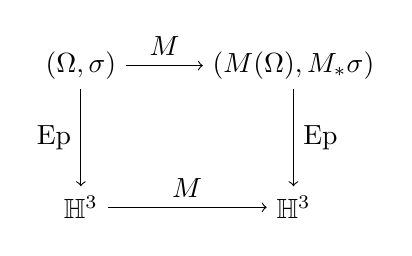
\begin{tikzpicture}[scale=0.9]
\node (1) at (0,2) {$(\Omega,\sigma)$};
\node (2) at (3,2) {$(M(\Omega),M_*\sigma)$};
\node (3) at (0,0) {$\H^3$};
\node (4) at (3,0) {$\H^3$};


\draw[->] (1) to node [above] {$M$} (2);
\draw[->] (1) to node [left] {$\mathrm{Ep}$} (3);
\draw[->] (3) to node [above] {$M$} (4);
\draw[->] (2) to node [right] {$\mathrm{Ep}$} (4);
\end{tikzpicture}
\]
That is, $\mathrm{Ep}_{M_*\sigma}(M(z)) = M( \mathrm{Ep}_{\sigma}(z))$. 
This is because both $M \circ \mathrm{Ep}_\sigma$ and $\mathrm{Ep}_{M_*\sigma} \circ M$ as maps on $\Omega$ satisfy the visual metric condition from Theorem \ref{epstein-map-def} (see \cite{anderson1998} for more details ).

This allows us to define Epstein maps on certain quotients. 
Suppose in general that $\Gamma$ is a subgroup of $\mathrm{SL}_2\C$ acting freely and properly discontinuously on $\H^3 \cup \CP^1$ leaving a domain $\Omega$ invariant. 
Then $\Omega/\Gamma$ inherits a Riemann surface structure. 
Call this structure $X$ and let $\sigma$ be a conformal metric  on $X$.
Lift this to $\tilde{\sigma}$ on $\Omega$, which is $\Gamma$-invariant. 
Then $\mathrm{Ep}_{\tilde{\sigma}}: \Omega \to \H^3$ is $\Gamma$-equivariant and therefore descends to a map $\mathrm{Ep}_\sigma : X \to \H^3/ \Gamma$. 
In particular, when $\Gamma$ is a quasi-Fuchsian group and $\Omega$ a component of the domain of discontinuity, each conformal metric $\sigma$ on the surface at infinity $X$ gives rise to a map from $X$ into the quasi-Fuchsian manifold $M$.

Uniqueness also shows us that the surfaces parallel to an Epstein surface are themselves Epstein surfaces. 
More specifically, let $g^t : U \H^3 \to \H^3$ denote the time-$t$ geodesic flow projected down to $\H^3$.
Thus for a unit tangent vector $v$ on $\H^3$ we have $g^t(v) = \exp_p(tv)$.
Using the lift of an Epstein surface to $U\H^3$ described above, each Epstein surface gives rise to a family of surfaces by applying the geodesic flow (and projecting to $\H^3$). 
That is, we have the flowed surfaces $g^t \circ \widehat{\mathrm{Ep}}_\sigma(\Omega)$. 
These surfaces are themselves Epstein surfaces corresponding to scalar multiples of $\sigma$. 
Indeed, since the parallel flow of a horosphere is a horosphere, we know $[g^t(\widehat{\mathrm{Ep}}_\sigma(z)),z] = [\mathrm{Ep}_\sigma(z),z] + t$. 
This shows us
\[
V_{g^t(\widehat{\mathrm{Ep}}_\sigma(z))}(z) = e^{2[g^t(\widehat{\mathrm{Ep}}_\sigma(z)),z]}\overset{\circ}{\sigma}(z) = e^{2t}e^{2[\mathrm{Ep}_\sigma(z),z]}\overset{\circ}{\sigma}(z) = e^{2t}\sigma(z).
\]
But the unique map that satisfies this equality is $\mathrm{Ep}_{e^{2t}\sigma}$. 
In summary, we have the following lemma, attributed to Thurston (unpublished work) by Epstein in \cite{epstein1984}.
\begin{lem}
\label{epstein-flow}
Let $\Omega$ be a domain in $\CP^1$ and $\sigma$ a conformal metric on $\Omega$.
Then 
\[
g^t \circ \widehat{\mathrm{Ep}}_\sigma  = \mathrm{Ep}_{e^{2t} \sigma}.
\]
That is, flowing the Epstein surface for $\sigma$ for time $t$ in the normal direction corresponds to taking the Epstein surface for the metric $e^{2t}\sigma$.
\end{lem}

\section{Geometry of Epstein surfaces}
\label{epstein-geometry}

The first fundamental form of the Epstein surface for the metric $\sigma$ is given by $I(\sigma) = \mathrm{Ep}_\sigma^*(g_{\H^3})$ for $g_{\H^3}$ the metric of $\H^3$. 
It is given by 
\[
I(\sigma) = 4|B(g_{\CP^1},\sigma)|^2\sigma^{-1} + \frac{1}{4}(1-K(\sigma))^2\sigma + 2(1-K(\sigma))\text{Re}(B(g_{\CP^1},\sigma)).
\]
The second fundamental form (relative to the normal lift $\widehat{\mathrm{Ep}}_\sigma$) is 
\[
\two(\sigma)
= 4|B(g_{\CP^1},\sigma)|^2\sigma^{-1} - \frac{1}{4} (1 - K(\sigma)^2)\sigma - 2 K(\sigma) \text{Re}(B(g_{\CP^1},\sigma)).
\]
These formulas are derived in \cite[Eqns.~3.2-3.3]{dumas2017}.
Here $K(\sigma)$ is the Gaussian curvature of $\sigma$ and $B(g_{\CP^1},\sigma)$ the Schwarzian derivative of $\sigma$ with respect to a M\"obius flat metric. 
We note that when the Epstein surface is embedded, its second fundamental form is negative definite due to our convenient choice of normal vector field.
Writing $\det(g)$ for the determinant of the matrix representation of $g$ relative to some local frame for the tangent bundle, the metrics on $\sigma$ and $I(\sigma)$ on $S$ have determinants related by
\[
\det(I(\sigma)) = \left( (1-K(\sigma))^2 - 16 |B(g_{\CP^1},\sigma)|^2\sigma^{-2} \right)^2 \det(\sigma).
\]
This equation is independent of the frame and has in intrinsic meaning, namely it describes the ratio of volume forms of these two metrics. 
We can compute the Gaussian curvature by $K(I(\sigma)) = -1 + \det(I(\sigma)^{-1}\two(\sigma))$ and the mean curvature by $H(\mathrm{Ep}_\sigma) = \frac{1}{2}\mathrm{tr}(I(\sigma)^{-1}\two(\sigma))$. 
We obtain
\[
K(I(\sigma))
= \frac{4K(\sigma)}{(1-K(\sigma))^2 - 16|B(g_{\CP^1},\sigma)|^2\sigma^{-2}}
\]
and
\[
H(\mathrm{Ep}_\sigma)
= \frac{K(\sigma)^2 - 1 - 16 |B(g_{\CP^1},\sigma)|^2\sigma^{-2}}{(K(\sigma) - 1)^2 - 16 |B(g_{\CP^1},\sigma)|^2\sigma^{-2}}.
\]

 
In the quasi-Fuchsian setting, if $\sigma$ is a $\Gamma$-invariant conformal metric on $\Omega$ then each term in the above equations is also $\Gamma$-invariant. 
This may be less clear for the quadratic differential $B(g_{\CP^1},\sigma)$ since the M\"obius flat metric $g_{\CP^1}$ is not itself $\Gamma$-invariant. 
However, we see that for $\gamma \in \Gamma$ we have $\gamma^*B(g_{\CP^1},\sigma) = B(\gamma^*g_{\CP^1},\gamma^*\sigma) = B(\gamma^* g_{\CP^1},\sigma)$, by naturality of Schwarzian derivatives of conformal metrics. 
The metric $\gamma^* g_{\CP^1}$ is still a M\"obius flat metric, and so $B(\gamma^* g_{\CP^1},\sigma) = B(g_{\CP^1},\sigma)$, implying $B(g_{\CP^1}, \sigma)$ is $\Gamma$-invariant. 
Therefore, $B(g_{\CP^1},\sigma)$ induces a quadratic differential on $X$, which we will denote by $B(\sigma)$.

In summary of the above, we have the following Gaussian and mean curvatures of the Epstein surfaces in $M$.
\begin{lem}
\label{curvature-epstein}
The Gaussian curvature for the Epstein surface $\mathrm{Ep}_\sigma : X \to M$ is given by
\[
K(I(\sigma))
= \frac{4K(\sigma)}{(1-K(\sigma))^2 - 16 |B(g_{\CP^1},\sigma)|^2\sigma^{-2}},
\]
and the mean curvature by 
\[
\pushQED{\qed}
H(\mathrm{Ep}_\sigma)
= \frac{K(\sigma)^2 - 1 - 16 |B(g_{\CP^1},\sigma)|^2\sigma^{-2}}{(K(\sigma) - 1)^2 - 16 |B(g_{\CP^1},\sigma)|^2\sigma^{-2}}.
\qedhere
\popQED
\]
\end{lem}
These are now equations on the compact Riemann surface $X$.

\chapter{Epstein Surfaces}
\label{epstein-surfaces}

\section{The visual metric construction}


A natural trivialization of the unit tangent bundle of hyperbolic space $U\H^3$ is given as
\[
U\H^3 \to \H^3 \times \CP^1
\quad \text{ by } \quad
(p,v) \mapsto (p, \lim_{t \to \infty} \exp_p (tv) ).
\]
That is we map $(p,v)$ to the ideal endpoint of the geodesic ray through $p$ in the direction $v$. 
Restricting to a point $p$ and using the diffeomorphism $U_p\H^3 \to \CP^1$, we can push forward to $\CP^1$ the induced metric on $U_p\H^3$ considered as a submanifold of $T_p\H^3$ with metric given by the inner product $g_{\H^3}(p)$. 
The resulting metric $V_p$ on $\CP^1$ is called the visual metric from $p$.
As an example, the visual metric from the origin in the ball model $V_0$ is just the spherical metric $\overset{\circ}{\sigma}$ on $S^2$ (which is identified with $\CP^1$ in this model). 
In general, if $M \in \mathrm{PSL}_2\C$ is an isometry taking $0$ to the point $p$, then $V_p = M_*V_0$. 

As the spherical metric belongs to the conformal class of $\CP^1$, we have that $V_0$ is a conformal metric. 
Since M\"obius transformations are biholomorphisms of $\CP^1$, each $V_p$ is also a conformal metric. 
If we work in the ball model of hyperbolic space $\H^3 \cong \mathbb{B}^3$ we can actually be explicit regarding the conformal factor between $V_p$ and $\overset{\circ}{\sigma}$ using the affine parameter of a horosphere. 
If $H$ is a horosphere, then its affine parameter is the signed hyperbolic distance from $0 \in \H^3$ to $H$, positive if $0$ is outside $H$ and negative if inside. 
Then for $p \in \H^3$ there is a unique horosphere based at $z \in \CP^1$ that contains $p$. 
Denote by $[p,z]$ the affine parameter of this horosphere. 
Then
\[
V_p(z) = e^{2[p,z]}\overset{\circ}{\sigma}(z).
\]

We now describe the Visual Metric Construction (see \cite{anderson1998}). 
This is a process that, given a strictly convex surface $S$ in $\H^3$, gives a domain $\Omega$ in $\CP^1$ and a conformal metric $\sigma$ on $\Omega$.
The idea is this: Given $S$, we have its image under the Gauss map on $\CP^1$. 
That is, given a unit normal vector field $n$ on $S$ for which $S$ is strictly convex, define
\[
\mathcal{G}:S \to \CP^1 \text{ by } \mathcal{G}(p) = \lim_{t \to \infty} \exp_p(t n(p)).
\]
The strict convexity of $S$ guarantees the map $\mathcal{G}$ is a local homeomorphism. 
We assume now that it is actually a homeomorphism.
The image surface also comes equipped with a metric $\sigma$ by defining $\sigma(\mathcal{G}(p)) = V_p(\mathcal{G}(p))$. 
Since for each $p$ the visual metric from $p$ is a conformal metric on $\CP^1$, we have $\sigma$ itself is a conformal metric. 

Epstein in \cite{epstein1984} describes an inverse process to the visual metric construction, which we describe below.

\section{The Epstein map}


As an inverse to the visual metric construction above, the Epstein map takes a domain $\Omega$ in $\CP^1$ and a conformal metric $\sigma$ on $\Omega$ and describes a strictly convex surface $f: \Omega \to \H^3$. 
This surface has the property that $V_{f(z)}(z) = \sigma(z)$ and this property can be used to derive a formula for the surface. 
Specifically, expanding upon this last condition and using the affine parameter discussed above, we see that 
\[
\sigma(z) = V_{f(z)}(z) = e^{2 [f(z),z]} \overset{\circ}{\sigma}(z),
\]
or that $f(z)$ lies on the horosphere based at $z$ with affine parameter
\[
[f(z),z] = \frac{1}{2} \log \left( \frac{\sigma(z)}{\overset{\circ}{\sigma}(z)} \right) =: \rho(z).
\]
Hence, we know which horosphere based at $z$ that $f(z)$ must lie on. 

There is a convenient choice of normal vector field. 
At $f(z)$, the geodesic in the direction $n(f(z))$ must end at $z$ in order for $f$ to be an inverse to the visual metric construction. 
The normal vectors to a horosphere pointing to its base have this property, so we define $n(f(z))$ to be the normal vector to the horosphere based at $z$ with affine parameter $\rho(z)$. 
Since $n$ must be normal to the image surface $S = f(\Omega)$, this identifies the tangent spaces to the sought-after $S$ with the tangent spaces to the horospheres. 
And this identifies the surface $S$ with the envelope of the family of horospheres
\[
\mathcal{H}(\Omega,\sigma) = \{ \text{Horosphere based at $z$ with parameter $\rho(z)$} \ | \ z \in \Omega \}.
\]


In \cite{epstein1984}, Epstein derives an equation for such an envelope. 
Working in the ball model and taking $z$ both as a point in $\CP^1 \cong S^2$ as well as a unit vector in $\R^3$, he shows the desired map is 
\[
\mathrm{Ep}_\sigma(z) = \frac{|\overset{\circ}{\nabla}\rho(z)|^2 + e^{2\rho(z)} - 1}{|\overset{\circ}{\nabla}\rho(z)|^2 + (e^{\rho(z)}+1)^2} z + \frac{2}{|\overset{\circ}{\nabla}\rho(z)|^2 + (e^{\rho(z)}+1)^2} \overset{\circ}{\nabla}\rho(z),
\]
where $\overset{\circ}{\nabla}\rho$ is the gradient of $\rho$ with respect to the spherical metric on $S^2$. 
This construction leads to the following theorem. 


\begin{thm}[Epstein \cite{epstein1984}]
Let $\Omega$ be a domain in $\CP^1$  and $\sigma$ a $C^k$ conformal metric on $\Omega$, then there exists a unique $C^{k-1}$ map $\mathrm{Ep}_\sigma : \Omega \to \H^3$, called the Epstein map of $\Omega$ for the metric $\sigma$, such that for all $z \in \Omega$,
\[
V_{\mathrm{Ep}_\sigma(z)}(z) = \sigma(z).
\]
Moreover, the image of a point $z$ depends only on the 1-jet of $\sigma$ at $z$.
\label{epstein-map-def}
\end{thm}

Epstein's original construction uses the ball model of hyperbolic space to define the Epstein map. 
In \cite{dumas2017}, Dumas gives a model independent definition of the map using an $\text{SL}_2\C$-frame field. 
It proceeds as follows. 
Choose an affine coordinate chart $z$ on $\CP^1$ that distinguishes a point $0 \in \Omega$ and $\infty \notin \Omega$. 
Then, on the geodesic in $\H^3$ with ideal endpoints $0$ and $\infty$, there exists a unique point $p$ such that the visual metric from $p$ at $0$ is the Euclidean metric of this affine chart, $V_p(0) = |dz|^2$. 
The Epstein map is an $\mathrm{SL}_2\C$-frame orbit of this point.     


\begin{prop}[\cite{dumas2017}]
On a domain $\Omega$ in $\CP^1$ write $\sigma = e^{2\eta}|dz|^2$. Define the $\mathrm{SL}_2,\C$-frame field $\widetilde{\mathrm{Ep}}_\sigma: \Omega \to \mathrm{SL}_2\C$ by 
\[
\widetilde{\mathrm{Ep}}_\sigma(z) =
\begin{pmatrix}
1 & z \\
0 & 1
\end{pmatrix}
\begin{pmatrix}
1 & 0 \\
\eta_z & 1
\end{pmatrix}
\begin{pmatrix}
e^{-\eta/2} & 0 \\
0 & e^{\eta/2}
\end{pmatrix},
\]
then the Epstein map is given by 
\[
\mathrm{Ep}_\sigma(z) = \widetilde{\mathrm{Ep}}_\sigma(z) \cdot p.
\]
\end{prop}

 

Even though we call the image an Epstein surface, the Epstein map need not be an immersion. 
Indeed, if $\sigma$ is itself a visual metric then the Epstein map for $\sigma$ is constant. 
However, the lift of $\mathrm{Ep}_\sigma$ from $\Omega$ to the unit tangent bundle of hyperbolic space given by 
\[
\widehat{\mathrm{Ep}}_\sigma(z) = (\text{Ep}_\sigma(z),z) 
\] 
is an immersion (here we are using the trivialization $U\H^3 \cong \H^3 \times \CP^1$ defined above). 
This lift can be thought of as providing a unit ``normal'' vector field for the Epstein surface even when the Epstein map is not an immersion. 
Indeed, this lift agrees with a unit normal vector field when the surface is immersed and so we will simply refer to it as the normal field from now on. 

Because the Epstein map is unique, it is natural with respect to the action of $\mathrm{SL}_2\C$ in the following sense. 
Suppose $M \in \mathrm{SL}_2\C$, then the following diagram commutes:
\[
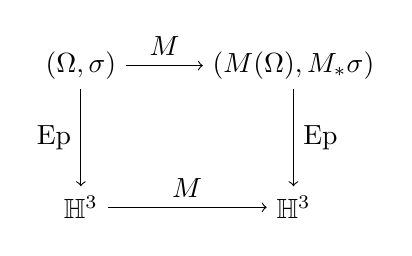
\begin{tikzpicture}[scale=0.9]
\node (1) at (0,2) {$(\Omega,\sigma)$};
\node (2) at (3,2) {$(M(\Omega),M_*\sigma)$};
\node (3) at (0,0) {$\H^3$};
\node (4) at (3,0) {$\H^3$};


\draw[->] (1) to node [above] {$M$} (2);
\draw[->] (1) to node [left] {$\mathrm{Ep}$} (3);
\draw[->] (3) to node [above] {$M$} (4);
\draw[->] (2) to node [right] {$\mathrm{Ep}$} (4);
\end{tikzpicture}
\]
That is, $\mathrm{Ep}_{M_*\sigma}(M(z)) = M( \mathrm{Ep}_{\sigma}(z))$. 
This is because both $M \circ \mathrm{Ep}_\sigma$ and $\mathrm{Ep}_{M_*\sigma} \circ M$ as maps on $\Omega$ satisfy the visual metric condition from Theorem \ref{epstein-map-def} (see \cite{anderson1998} for more details ).

This allows us to define Epstein maps on certain quotients. 
Suppose in general that $\Gamma$ is a subgroup of $\mathrm{SL}_2\C$ acting freely and properly discontinuously on $\H^3 \cup \CP^1$ leaving a domain $\Omega$ invariant. 
Then $\Omega/\Gamma$ inherits a Riemann surface structure. 
Call this structure $X$ and let $\sigma$ be a conformal metric  on $X$.
Lift this to $\tilde{\sigma}$ on $\Omega$, which is $\Gamma$-invariant. 
Then $\mathrm{Ep}_{\tilde{\sigma}}: \Omega \to \H^3$ is $\Gamma$-equivariant and therefore descends to a map $\mathrm{Ep}_\sigma : X \to \H^3/ \Gamma$. 
In particular, when $\Gamma$ is a quasi-Fuchsian group and $\Omega$ a component of the domain of discontinuity, each conformal metric $\sigma$ on the surface at infinity $X$ gives rise to a map from $X$ into the quasi-Fuchsian manifold $M$.

Uniqueness also shows us that the surfaces parallel to an Epstein surface are themselves Epstein surfaces. 
More specifically, let $g^t : U \H^3 \to \H^3$ denote the time-$t$ geodesic flow projected down to $\H^3$.
Thus for a unit tangent vector $v$ on $\H^3$ we have $g^t(v) = \exp_p(tv)$.
Using the lift of an Epstein surface to $U\H^3$ described above, each Epstein surface gives rise to a family of surfaces by applying the geodesic flow (and projecting to $\H^3$). 
That is, we have the flowed surfaces $g^t \circ \widehat{\mathrm{Ep}}_\sigma(\Omega)$. 
These surfaces are themselves Epstein surfaces corresponding to scalar multiples of $\sigma$. 
Indeed, since the parallel flow of a horosphere is a horosphere, we know $[g^t(\widehat{\mathrm{Ep}}_\sigma(z)),z] = [\mathrm{Ep}_\sigma(z),z] + t$. 
This shows us
\[
V_{g^t(\widehat{\mathrm{Ep}}_\sigma(z))}(z) = e^{2[g^t(\widehat{\mathrm{Ep}}_\sigma(z)),z]}\overset{\circ}{\sigma}(z) = e^{2t}e^{2[\mathrm{Ep}_\sigma(z),z]}\overset{\circ}{\sigma}(z) = e^{2t}\sigma(z).
\]
But the unique map that satisfies this equality is $\mathrm{Ep}_{e^{2t}\sigma}$. 
In summary, we have the following lemma, attributed to Thurston (unpublished work) by Epstein in \cite{epstein1984}.
\begin{lem}
\label{epstein-flow}
Let $\Omega$ be a domain in $\CP^1$ and $\sigma$ a conformal metric on $\Omega$.
Then 
\[
g^t \circ \widehat{\mathrm{Ep}}_\sigma  = \mathrm{Ep}_{e^{2t} \sigma}.
\]
That is, flowing the Epstein surface for $\sigma$ for time $t$ in the normal direction corresponds to taking the Epstein surface for the metric $e^{2t}\sigma$.
\end{lem}

\section{Geometry of Epstein surfaces}
\label{epstein-geometry}

The first fundamental form of the Epstein surface for the metric $\sigma$ is given by $I(\sigma) = \mathrm{Ep}_\sigma^*(g_{\H^3})$ for $g_{\H^3}$ the metric of $\H^3$. 
It is given by 
\[
I(\sigma) = 4|B(g_{\CP^1},\sigma)|^2\sigma^{-1} + \frac{1}{4}(1-K(\sigma))^2\sigma + 2(1-K(\sigma))\text{Re}(B(g_{\CP^1},\sigma)).
\]
The second fundamental form (relative to the normal lift $\widehat{\mathrm{Ep}}_\sigma$) is 
\[
\two(\sigma)
= 4|B(g_{\CP^1},\sigma)|^2\sigma^{-1} - \frac{1}{4} (1 - K(\sigma)^2)\sigma - 2 K(\sigma) \text{Re}(B(g_{\CP^1},\sigma)).
\]
These formulas are derived in \cite[Eqns.~3.2-3.3]{dumas2017}.
Here $K(\sigma)$ is the Gaussian curvature of $\sigma$ and $B(g_{\CP^1},\sigma)$ the Schwarzian derivative of $\sigma$ with respect to a M\"obius flat metric. 
We note that when the Epstein surface is embedded, its second fundamental form is negative definite due to our convenient choice of normal vector field.
Writing $\det(g)$ for the determinant of the matrix representation of $g$ relative to some local frame for the tangent bundle, the metrics on $\sigma$ and $I(\sigma)$ on $S$ have determinants related by
\[
\det(I(\sigma)) = \left( (1-K(\sigma))^2 - 16 |B(g_{\CP^1},\sigma)|^2\sigma^{-2} \right)^2 \det(\sigma).
\]
This equation is independent of the frame and has in intrinsic meaning, namely it describes the ratio of volume forms of these two metrics. 
We can compute the Gaussian curvature by $K(I(\sigma)) = -1 + \det(I(\sigma)^{-1}\two(\sigma))$ and the mean curvature by $H(\mathrm{Ep}_\sigma) = \frac{1}{2}\mathrm{tr}(I(\sigma)^{-1}\two(\sigma))$. 
We obtain
\[
K(I(\sigma))
= \frac{4K(\sigma)}{(1-K(\sigma))^2 - 16|B(g_{\CP^1},\sigma)|^2\sigma^{-2}}
\]
and
\[
H(\mathrm{Ep}_\sigma)
= \frac{K(\sigma)^2 - 1 - 16 |B(g_{\CP^1},\sigma)|^2\sigma^{-2}}{(K(\sigma) - 1)^2 - 16 |B(g_{\CP^1},\sigma)|^2\sigma^{-2}}.
\]

 
In the quasi-Fuchsian setting, if $\sigma$ is a $\Gamma$-invariant conformal metric on $\Omega$ then each term in the above equations is also $\Gamma$-invariant. 
This may be less clear for the quadratic differential $B(g_{\CP^1},\sigma)$ since the M\"obius flat metric $g_{\CP^1}$ is not itself $\Gamma$-invariant. 
However, we see that for $\gamma \in \Gamma$ we have $\gamma^*B(g_{\CP^1},\sigma) = B(\gamma^*g_{\CP^1},\gamma^*\sigma) = B(\gamma^* g_{\CP^1},\sigma)$, by naturality of Schwarzian derivatives of conformal metrics. 
The metric $\gamma^* g_{\CP^1}$ is still a M\"obius flat metric, and so $B(\gamma^* g_{\CP^1},\sigma) = B(g_{\CP^1},\sigma)$, implying $B(g_{\CP^1}, \sigma)$ is $\Gamma$-invariant. 
Therefore, $B(g_{\CP^1},\sigma)$ induces a quadratic differential on $X$, which we will denote by $B(\sigma)$.

In summary of the above, we have the following Gaussian and mean curvatures of the Epstein surfaces in $M$.
\begin{lem}
\label{curvature-epstein}
The Gaussian curvature for the Epstein surface $\mathrm{Ep}_\sigma : X \to M$ is given by
\[
K(I(\sigma))
= \frac{4K(\sigma)}{(1-K(\sigma))^2 - 16 |B(g_{\CP^1},\sigma)|^2\sigma^{-2}},
\]
and the mean curvature by 
\[
\pushQED{\qed}
H(\mathrm{Ep}_\sigma)
= \frac{K(\sigma)^2 - 1 - 16 |B(g_{\CP^1},\sigma)|^2\sigma^{-2}}{(K(\sigma) - 1)^2 - 16 |B(g_{\CP^1},\sigma)|^2\sigma^{-2}}.
\qedhere
\popQED
\]
\end{lem}
These are now equations on the compact Riemann surface $X$.

\chapter{Epstein Surfaces}
\label{epstein-surfaces}

\section{The visual metric construction}


A natural trivialization of the unit tangent bundle of hyperbolic space $U\H^3$ is given as
\[
U\H^3 \to \H^3 \times \CP^1
\quad \text{ by } \quad
(p,v) \mapsto (p, \lim_{t \to \infty} \exp_p (tv) ).
\]
That is we map $(p,v)$ to the ideal endpoint of the geodesic ray through $p$ in the direction $v$. 
Restricting to a point $p$ and using the diffeomorphism $U_p\H^3 \to \CP^1$, we can push forward to $\CP^1$ the induced metric on $U_p\H^3$ considered as a submanifold of $T_p\H^3$ with metric given by the inner product $g_{\H^3}(p)$. 
The resulting metric $V_p$ on $\CP^1$ is called the visual metric from $p$.
As an example, the visual metric from the origin in the ball model $V_0$ is just the spherical metric $\overset{\circ}{\sigma}$ on $S^2$ (which is identified with $\CP^1$ in this model). 
In general, if $M \in \mathrm{PSL}_2\C$ is an isometry taking $0$ to the point $p$, then $V_p = M_*V_0$. 

As the spherical metric belongs to the conformal class of $\CP^1$, we have that $V_0$ is a conformal metric. 
Since M\"obius transformations are biholomorphisms of $\CP^1$, each $V_p$ is also a conformal metric. 
If we work in the ball model of hyperbolic space $\H^3 \cong \mathbb{B}^3$ we can actually be explicit regarding the conformal factor between $V_p$ and $\overset{\circ}{\sigma}$ using the affine parameter of a horosphere. 
If $H$ is a horosphere, then its affine parameter is the signed hyperbolic distance from $0 \in \H^3$ to $H$, positive if $0$ is outside $H$ and negative if inside. 
Then for $p \in \H^3$ there is a unique horosphere based at $z \in \CP^1$ that contains $p$. 
Denote by $[p,z]$ the affine parameter of this horosphere. 
Then
\[
V_p(z) = e^{2[p,z]}\overset{\circ}{\sigma}(z).
\]

We now describe the Visual Metric Construction (see \cite{anderson1998}). 
This is a process that, given a strictly convex surface $S$ in $\H^3$, gives a domain $\Omega$ in $\CP^1$ and a conformal metric $\sigma$ on $\Omega$.
The idea is this: Given $S$, we have its image under the Gauss map on $\CP^1$. 
That is, given a unit normal vector field $n$ on $S$ for which $S$ is strictly convex, define
\[
\mathcal{G}:S \to \CP^1 \text{ by } \mathcal{G}(p) = \lim_{t \to \infty} \exp_p(t n(p)).
\]
The strict convexity of $S$ guarantees the map $\mathcal{G}$ is a local homeomorphism. 
We assume now that it is actually a homeomorphism.
The image surface also comes equipped with a metric $\sigma$ by defining $\sigma(\mathcal{G}(p)) = V_p(\mathcal{G}(p))$. 
Since for each $p$ the visual metric from $p$ is a conformal metric on $\CP^1$, we have $\sigma$ itself is a conformal metric. 

Epstein in \cite{epstein1984} describes an inverse process to the visual metric construction, which we describe below.

\section{The Epstein map}


As an inverse to the visual metric construction above, the Epstein map takes a domain $\Omega$ in $\CP^1$ and a conformal metric $\sigma$ on $\Omega$ and describes a strictly convex surface $f: \Omega \to \H^3$. 
This surface has the property that $V_{f(z)}(z) = \sigma(z)$ and this property can be used to derive a formula for the surface. 
Specifically, expanding upon this last condition and using the affine parameter discussed above, we see that 
\[
\sigma(z) = V_{f(z)}(z) = e^{2 [f(z),z]} \overset{\circ}{\sigma}(z),
\]
or that $f(z)$ lies on the horosphere based at $z$ with affine parameter
\[
[f(z),z] = \frac{1}{2} \log \left( \frac{\sigma(z)}{\overset{\circ}{\sigma}(z)} \right) =: \rho(z).
\]
Hence, we know which horosphere based at $z$ that $f(z)$ must lie on. 

There is a convenient choice of normal vector field. 
At $f(z)$, the geodesic in the direction $n(f(z))$ must end at $z$ in order for $f$ to be an inverse to the visual metric construction. 
The normal vectors to a horosphere pointing to its base have this property, so we define $n(f(z))$ to be the normal vector to the horosphere based at $z$ with affine parameter $\rho(z)$. 
Since $n$ must be normal to the image surface $S = f(\Omega)$, this identifies the tangent spaces to the sought-after $S$ with the tangent spaces to the horospheres. 
And this identifies the surface $S$ with the envelope of the family of horospheres
\[
\mathcal{H}(\Omega,\sigma) = \{ \text{Horosphere based at $z$ with parameter $\rho(z)$} \ | \ z \in \Omega \}.
\]


In \cite{epstein1984}, Epstein derives an equation for such an envelope. 
Working in the ball model and taking $z$ both as a point in $\CP^1 \cong S^2$ as well as a unit vector in $\R^3$, he shows the desired map is 
\[
\mathrm{Ep}_\sigma(z) = \frac{|\overset{\circ}{\nabla}\rho(z)|^2 + e^{2\rho(z)} - 1}{|\overset{\circ}{\nabla}\rho(z)|^2 + (e^{\rho(z)}+1)^2} z + \frac{2}{|\overset{\circ}{\nabla}\rho(z)|^2 + (e^{\rho(z)}+1)^2} \overset{\circ}{\nabla}\rho(z),
\]
where $\overset{\circ}{\nabla}\rho$ is the gradient of $\rho$ with respect to the spherical metric on $S^2$. 
This construction leads to the following theorem. 


\begin{thm}[Epstein \cite{epstein1984}]
Let $\Omega$ be a domain in $\CP^1$  and $\sigma$ a $C^k$ conformal metric on $\Omega$, then there exists a unique $C^{k-1}$ map $\mathrm{Ep}_\sigma : \Omega \to \H^3$, called the Epstein map of $\Omega$ for the metric $\sigma$, such that for all $z \in \Omega$,
\[
V_{\mathrm{Ep}_\sigma(z)}(z) = \sigma(z).
\]
Moreover, the image of a point $z$ depends only on the 1-jet of $\sigma$ at $z$.
\label{epstein-map-def}
\end{thm}

Epstein's original construction uses the ball model of hyperbolic space to define the Epstein map. 
In \cite{dumas2017}, Dumas gives a model independent definition of the map using an $\text{SL}_2\C$-frame field. 
It proceeds as follows. 
Choose an affine coordinate chart $z$ on $\CP^1$ that distinguishes a point $0 \in \Omega$ and $\infty \notin \Omega$. 
Then, on the geodesic in $\H^3$ with ideal endpoints $0$ and $\infty$, there exists a unique point $p$ such that the visual metric from $p$ at $0$ is the Euclidean metric of this affine chart, $V_p(0) = |dz|^2$. 
The Epstein map is an $\mathrm{SL}_2\C$-frame orbit of this point.     


\begin{prop}[\cite{dumas2017}]
On a domain $\Omega$ in $\CP^1$ write $\sigma = e^{2\eta}|dz|^2$. Define the $\mathrm{SL}_2,\C$-frame field $\widetilde{\mathrm{Ep}}_\sigma: \Omega \to \mathrm{SL}_2\C$ by 
\[
\widetilde{\mathrm{Ep}}_\sigma(z) =
\begin{pmatrix}
1 & z \\
0 & 1
\end{pmatrix}
\begin{pmatrix}
1 & 0 \\
\eta_z & 1
\end{pmatrix}
\begin{pmatrix}
e^{-\eta/2} & 0 \\
0 & e^{\eta/2}
\end{pmatrix},
\]
then the Epstein map is given by 
\[
\mathrm{Ep}_\sigma(z) = \widetilde{\mathrm{Ep}}_\sigma(z) \cdot p.
\]
\end{prop}

 

Even though we call the image an Epstein surface, the Epstein map need not be an immersion. 
Indeed, if $\sigma$ is itself a visual metric then the Epstein map for $\sigma$ is constant. 
However, the lift of $\mathrm{Ep}_\sigma$ from $\Omega$ to the unit tangent bundle of hyperbolic space given by 
\[
\widehat{\mathrm{Ep}}_\sigma(z) = (\text{Ep}_\sigma(z),z) 
\] 
is an immersion (here we are using the trivialization $U\H^3 \cong \H^3 \times \CP^1$ defined above). 
This lift can be thought of as providing a unit ``normal'' vector field for the Epstein surface even when the Epstein map is not an immersion. 
Indeed, this lift agrees with a unit normal vector field when the surface is immersed and so we will simply refer to it as the normal field from now on. 

Because the Epstein map is unique, it is natural with respect to the action of $\mathrm{SL}_2\C$ in the following sense. 
Suppose $M \in \mathrm{SL}_2\C$, then the following diagram commutes:
\[
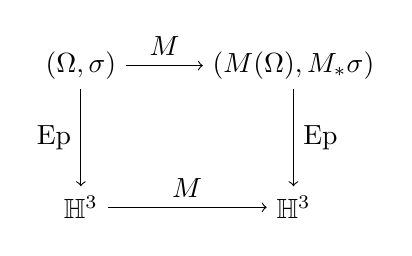
\begin{tikzpicture}[scale=0.9]
\node (1) at (0,2) {$(\Omega,\sigma)$};
\node (2) at (3,2) {$(M(\Omega),M_*\sigma)$};
\node (3) at (0,0) {$\H^3$};
\node (4) at (3,0) {$\H^3$};


\draw[->] (1) to node [above] {$M$} (2);
\draw[->] (1) to node [left] {$\mathrm{Ep}$} (3);
\draw[->] (3) to node [above] {$M$} (4);
\draw[->] (2) to node [right] {$\mathrm{Ep}$} (4);
\end{tikzpicture}
\]
That is, $\mathrm{Ep}_{M_*\sigma}(M(z)) = M( \mathrm{Ep}_{\sigma}(z))$. 
This is because both $M \circ \mathrm{Ep}_\sigma$ and $\mathrm{Ep}_{M_*\sigma} \circ M$ as maps on $\Omega$ satisfy the visual metric condition from Theorem \ref{epstein-map-def} (see \cite{anderson1998} for more details ).

This allows us to define Epstein maps on certain quotients. 
Suppose in general that $\Gamma$ is a subgroup of $\mathrm{SL}_2\C$ acting freely and properly discontinuously on $\H^3 \cup \CP^1$ leaving a domain $\Omega$ invariant. 
Then $\Omega/\Gamma$ inherits a Riemann surface structure. 
Call this structure $X$ and let $\sigma$ be a conformal metric  on $X$.
Lift this to $\tilde{\sigma}$ on $\Omega$, which is $\Gamma$-invariant. 
Then $\mathrm{Ep}_{\tilde{\sigma}}: \Omega \to \H^3$ is $\Gamma$-equivariant and therefore descends to a map $\mathrm{Ep}_\sigma : X \to \H^3/ \Gamma$. 
In particular, when $\Gamma$ is a quasi-Fuchsian group and $\Omega$ a component of the domain of discontinuity, each conformal metric $\sigma$ on the surface at infinity $X$ gives rise to a map from $X$ into the quasi-Fuchsian manifold $M$.

Uniqueness also shows us that the surfaces parallel to an Epstein surface are themselves Epstein surfaces. 
More specifically, let $g^t : U \H^3 \to \H^3$ denote the time-$t$ geodesic flow projected down to $\H^3$.
Thus for a unit tangent vector $v$ on $\H^3$ we have $g^t(v) = \exp_p(tv)$.
Using the lift of an Epstein surface to $U\H^3$ described above, each Epstein surface gives rise to a family of surfaces by applying the geodesic flow (and projecting to $\H^3$). 
That is, we have the flowed surfaces $g^t \circ \widehat{\mathrm{Ep}}_\sigma(\Omega)$. 
These surfaces are themselves Epstein surfaces corresponding to scalar multiples of $\sigma$. 
Indeed, since the parallel flow of a horosphere is a horosphere, we know $[g^t(\widehat{\mathrm{Ep}}_\sigma(z)),z] = [\mathrm{Ep}_\sigma(z),z] + t$. 
This shows us
\[
V_{g^t(\widehat{\mathrm{Ep}}_\sigma(z))}(z) = e^{2[g^t(\widehat{\mathrm{Ep}}_\sigma(z)),z]}\overset{\circ}{\sigma}(z) = e^{2t}e^{2[\mathrm{Ep}_\sigma(z),z]}\overset{\circ}{\sigma}(z) = e^{2t}\sigma(z).
\]
But the unique map that satisfies this equality is $\mathrm{Ep}_{e^{2t}\sigma}$. 
In summary, we have the following lemma, attributed to Thurston (unpublished work) by Epstein in \cite{epstein1984}.
\begin{lem}
\label{epstein-flow}
Let $\Omega$ be a domain in $\CP^1$ and $\sigma$ a conformal metric on $\Omega$.
Then 
\[
g^t \circ \widehat{\mathrm{Ep}}_\sigma  = \mathrm{Ep}_{e^{2t} \sigma}.
\]
That is, flowing the Epstein surface for $\sigma$ for time $t$ in the normal direction corresponds to taking the Epstein surface for the metric $e^{2t}\sigma$.
\end{lem}

\section{Geometry of Epstein surfaces}
\label{epstein-geometry}

The first fundamental form of the Epstein surface for the metric $\sigma$ is given by $I(\sigma) = \mathrm{Ep}_\sigma^*(g_{\H^3})$ for $g_{\H^3}$ the metric of $\H^3$. 
It is given by 
\[
I(\sigma) = 4|B(g_{\CP^1},\sigma)|^2\sigma^{-1} + \frac{1}{4}(1-K(\sigma))^2\sigma + 2(1-K(\sigma))\text{Re}(B(g_{\CP^1},\sigma)).
\]
The second fundamental form (relative to the normal lift $\widehat{\mathrm{Ep}}_\sigma$) is 
\[
\two(\sigma)
= 4|B(g_{\CP^1},\sigma)|^2\sigma^{-1} - \frac{1}{4} (1 - K(\sigma)^2)\sigma - 2 K(\sigma) \text{Re}(B(g_{\CP^1},\sigma)).
\]
These formulas are derived in \cite[Eqns.~3.2-3.3]{dumas2017}.
Here $K(\sigma)$ is the Gaussian curvature of $\sigma$ and $B(g_{\CP^1},\sigma)$ the Schwarzian derivative of $\sigma$ with respect to a M\"obius flat metric. 
We note that when the Epstein surface is embedded, its second fundamental form is negative definite due to our convenient choice of normal vector field.
Writing $\det(g)$ for the determinant of the matrix representation of $g$ relative to some local frame for the tangent bundle, the metrics on $\sigma$ and $I(\sigma)$ on $S$ have determinants related by
\[
\det(I(\sigma)) = \left( (1-K(\sigma))^2 - 16 |B(g_{\CP^1},\sigma)|^2\sigma^{-2} \right)^2 \det(\sigma).
\]
This equation is independent of the frame and has in intrinsic meaning, namely it describes the ratio of volume forms of these two metrics. 
We can compute the Gaussian curvature by $K(I(\sigma)) = -1 + \det(I(\sigma)^{-1}\two(\sigma))$ and the mean curvature by $H(\mathrm{Ep}_\sigma) = \frac{1}{2}\mathrm{tr}(I(\sigma)^{-1}\two(\sigma))$. 
We obtain
\[
K(I(\sigma))
= \frac{4K(\sigma)}{(1-K(\sigma))^2 - 16|B(g_{\CP^1},\sigma)|^2\sigma^{-2}}
\]
and
\[
H(\mathrm{Ep}_\sigma)
= \frac{K(\sigma)^2 - 1 - 16 |B(g_{\CP^1},\sigma)|^2\sigma^{-2}}{(K(\sigma) - 1)^2 - 16 |B(g_{\CP^1},\sigma)|^2\sigma^{-2}}.
\]

 
In the quasi-Fuchsian setting, if $\sigma$ is a $\Gamma$-invariant conformal metric on $\Omega$ then each term in the above equations is also $\Gamma$-invariant. 
This may be less clear for the quadratic differential $B(g_{\CP^1},\sigma)$ since the M\"obius flat metric $g_{\CP^1}$ is not itself $\Gamma$-invariant. 
However, we see that for $\gamma \in \Gamma$ we have $\gamma^*B(g_{\CP^1},\sigma) = B(\gamma^*g_{\CP^1},\gamma^*\sigma) = B(\gamma^* g_{\CP^1},\sigma)$, by naturality of Schwarzian derivatives of conformal metrics. 
The metric $\gamma^* g_{\CP^1}$ is still a M\"obius flat metric, and so $B(\gamma^* g_{\CP^1},\sigma) = B(g_{\CP^1},\sigma)$, implying $B(g_{\CP^1}, \sigma)$ is $\Gamma$-invariant. 
Therefore, $B(g_{\CP^1},\sigma)$ induces a quadratic differential on $X$, which we will denote by $B(\sigma)$.

In summary of the above, we have the following Gaussian and mean curvatures of the Epstein surfaces in $M$.
\begin{lem}
\label{curvature-epstein}
The Gaussian curvature for the Epstein surface $\mathrm{Ep}_\sigma : X \to M$ is given by
\[
K(I(\sigma))
= \frac{4K(\sigma)}{(1-K(\sigma))^2 - 16 |B(g_{\CP^1},\sigma)|^2\sigma^{-2}},
\]
and the mean curvature by 
\[
\pushQED{\qed}
H(\mathrm{Ep}_\sigma)
= \frac{K(\sigma)^2 - 1 - 16 |B(g_{\CP^1},\sigma)|^2\sigma^{-2}}{(K(\sigma) - 1)^2 - 16 |B(g_{\CP^1},\sigma)|^2\sigma^{-2}}.
\qedhere
\popQED
\]
\end{lem}
These are now equations on the compact Riemann surface $X$.


% No need to make any changes to this file below this line.
\newpage
\bibformb
\bibliography{thesis}
%\bibliographystyle{alpha}
\newpage
\vita
\begin{singlespace}
 \hspace{-12pt}{\bf \LARGE Keaton Quinn}\\ \\
\indent Department of Mathematics, Statistics, and Computer Science \\
\indent University of Illinois at Chicago \\
\indent \href{http://www.math.uic.edu/~kquinn23}{math.uic.edu/$\sim$kquinn23}\\
\indent \href{mailto:kquinn23@uic.edu}{kquinn23@uic.edu} \\ 






\vfill

\vspace{5pt}
\hspace{-12pt}{\color{sectiontitles}{\large Education}}
\vspace{10pt}

{\bf University of Illinois at Chicago} \hfill { Candidate}

Department of Mathematics, Statistics, and Computer Science

Ph.D., Mathematics

Advisor: David Dumas
\\

{\bf Michigan State University} \hfill {May 2014} 

Lyman Briggs College, Honors College

B.S., Mathematics, Advanced, with High Honors \\

\vfill

\vspace{5pt}
\hspace{-12pt}{\color{sectiontitles}{\large Awards and Honors}}
\vspace{10pt}



	{RTG Pre-Doctoral Fellowship} \hfill{Fall 2014, Spring 2015, Summer 2018} \\
	\indent \indent{\em Department of MSCS, UIC}
	
	{Academic Excellence Award} \hfill{May 2014}\\
	\indent \indent{\em Lyman Briggs College, MSU}
	
	{Teaching Assistant Award (Honorable Mention)} \hfill{April 2014} \\
	\indent \indent{\em Department of Mathematics, MSU}
	
	{Paul and Wilma Dressel Endowed Scholarship} \hfill{April 2013} \\
	\indent \indent{\em Department of Mathematics, MSU}

	{Paul and Gertrude Parker Scholarship} \hfill {April 2011} \\
	\indent \indent{\em Lyman Briggs College, MSU}
	
	{Doctor Ronald C Hamelink Scholarship} \hfill {December 2010} \\
	\indent \indent{\em Lyman Briggs College, MSU} \\


\vfill

\vspace{5pt}
\hspace{-12pt}{\color{sectiontitles}{\large Publications}}
\vspace{10pt}

%{\bf Submitted:}

%{\bf Accepted}

Asymptotically Poincar\'e surfaces in quasi-Fuchsian manifolds. \underline{Proc. Amer. Math. Soc.}, \indent 148:1239-1253, 2020.

\vfill

\vspace{5pt}
\hspace{-12pt}{\color{sectiontitles}{\large Talks and Presentations}}
\vspace{10pt}

{\em Limits of $k$-surfaces} \hfill {May 2019} \\
\indent \indent{Geometry and Topology Seminar, University of Luxembourg}

{\em An Introduction to Differential Geometry} \hfill {February 2018} \\
\indent \indent{Math Graduate Student Colloquium, UIC}

{\em The Many Flavors of Teichm\"uller Space} \hfill {March 2017} \\
\indent \indent{Math Graduate Student Colloquium, UIC}

{\em Inverse Modeling of Dynamical Systems} \hfill {August 2011}\\
\indent \indent{Michigan Mathematics REU Conference, Hope College} \\

\vfill

\vspace{5pt}
\hspace{-12pt}{\color{sectiontitles}{\large Organization}}
\vspace{10pt}


{\bf Conferences:}

\href{https://www.math.uic.edu/gstgc2018/}{Graduate Student Topology and Geometry Conference 2018}	 \hfill 
{April 7-8, 2018}


\href{https://sites.google.com/a/uic.edu/chicago-area-siam-student-conference-2016/home}{Chicago Area SIAM Student Conference}	 \hfill  {April 16, 2016} \\

{\bf Seminars:}

 
 \href{}{Spectra Student Chapter Seminar (for LGBT graduate students)} \hfill {2019 -- Present}

 \href{}{Out in Math Seminar (for LGBT graduate students)} \hfill {2018 -- 2019}
 
 \href{}{UIC Graduate Geometry, Topology, and Dynamics Seminar}	 \hfill  {2018 -- 2019} \\


\vfill

\vspace{5pt}
\hspace{-12pt}{\color{sectiontitles}{\large Service}}
\vspace{10pt}


{AMS Secretary} \hfill {September 2016 -- May 2019} \\
\indent \indent{\em UIC AMS Student Chapter} 

{SIAM Secretary} \hfill {September 2015 -- May 2016} \\
\indent \indent {\em UIC SIAM Student Chapter} 

{QED Youth Math Symposium Judge} \hfill {December 2015} \\
\indent \indent {\em Math Circles of Chicago}

{Math Learning Center (Neighborhood) Supervisor} \hfill {August 2013 -- May 2014}\\
\indent \indent {\em Department of Mathematics, MSU} \\

\vfill

\vspace{5pt}
\hspace{-12pt}{\color{sectiontitles}{\large Teaching}}
\vspace{10pt}


{\bf University of Illinois at Chicago} \\
\indent {\em Instructor:}

MATH 090, Summer Enrichment Workshop College Algebra \hfill Summer 2016, 2019

MATH 179, Emerging Scholars Program (ESP) Calculus I \hfill Fall 2015 

MATH 182, ESP Calculus II \hfill Spring 2016 

MATH 211, ESP Calculus III \hfill Spring 2018, Fall 2018, Fall 2019

MATH 294, ESP Intro. to Advanced Mathematics \hfill Fall 2016, Spring 2017, Fall 2017\\

\indent {\em Teaching Assistant:}

Asian American Resource and Cultural Center Tutor \hfill Fall 2017\\

\indent{\em Grader:}

MATH 215, Introduction to Advanced Mathematics \hfill Spring 2015, Fall 2016

MATH 417, Complex Analysis \hfill Fall 2019

MATH 547, Algebraic Topology I \hfill Fall 2016

MATH 549, Differentiable Manifolds I \hfill Spring 2017\\

{\bf College of Osteopathic Medicine, MSU}

OsteoCHAMPS Math Instructor \hfill Summer 2014\\


{\bf Michigan State Univeristy}\\
\indent {\em Teaching Assistant:}

LB 118, Calculus I \hfill Spring 2011, Spring 2012 

LB 119, Calculus II \hfill Spring 2013, Fall 2013, Spring 2014

LB 220, Calculus III \hfill Fall 2011, Fall 2012

MTH 153H, Honors Calculus II \hfill Fall 2013 

MTH 299, Transitions \hfill Fall 2013, Spring 2014

MTH 317H, Honors Linear Algebra \hfill Spring 2014 \\


\vspace{5pt}
\hspace{-12pt}{\color{sectiontitles}{\large Affiliations}}
\vspace{10pt}

United States Citizen

AMS

SIAM

Phi Beta Kappa

\end{singlespace}

\end{document}